\chapter{颈部}

\section{检查方法}

\subsection{常用的扫描方法}

\subsubsection{平扫}

①横断面扫描,病人仰卧,颈部略垫高,头稍后仰,且使颈部尽量与扫描线垂直。两臂放于身体两侧并尽量下垂。常规扫描应包括整个颈部,层厚和间隔为10mm;病变区特别是小病灶区可选用2~5mm薄层。针对某一脏器如甲状腺应直接选用5mm层厚为宜。②上颈部近颅底特别是口腔病变,可直接冠状面扫描,多选用3~5mm层厚和间隔。

\subsubsection{增强扫描}

有利于显示血管结构和小病灶。采用静脉快速注射(团注法)碘造影剂50~100ml,扫描范围同平扫。根据扫描方式可分为:①普通增强扫描;②连续动态扫描即动床式动态扫描;③同层动态扫描。

\subsubsection{螺旋CT扫描}

其增强扫描效果好,血管清晰,易于和淋巴结区分,并可行三维重建。一般情况下可采用5~10mm准直(层厚),延时15~20秒,对比剂用量80~100ml,流率3ml/s。

\subsubsection{发声时CT检查、椎管造影CT检查等}

\subsection{颈动脉螺旋CT血管成像}

螺旋CT血管成像(SCTA)对颈动脉病变如动脉瘤、狭窄、中老年人的颈动脉分叉扩张症等的诊断价值日趋重要。扫描前需确定以下参数:准直宽度(层厚)、螺距、扫描时间、对比剂剂量、注射流率及延迟时间。扫描方向自下向上,99%的颈动脉分叉位于C\textsubscript{6}
~C\textsubscript{3}
之间。如欲行颈动脉内膜切除术,应加大螺距值,增加扫描范围,并增加对比剂用量。

常用扫描层厚为3mm,重建间隔为1mm(多层螺旋CT可用更薄的有效层厚和重建间隔)。一般延时15~20秒。常用对比剂用量90~150ml(多采用120ml),流率为3~5ml/s。但国内复旦大学中山医院的研究认为,流率超过4ml/s不仅无明显实际意义,而且导致扫描出现伪影;造影剂用量应按下列公式计算:造影剂总量=注射流率×(扫描延迟时间+扫描持续时间-5),因为对比剂从肘静脉进入左心至少需5秒。

三维血管重建一般采用SSD、MIP。重建的三维血管图像可旋转,既可单独显示血管结构,亦可加骨标志,还能做血管CTVE。

\section{正常解剖和CT表现}

\subsection{颈部的临床分区}

颈部上方以下颌骨下缘、上项线、枕外粗隆的连线与头部为界,下缘以胸骨颈静脉切迹、锁骨、肩胛骨肩峰至C\textsubscript{7}
棘突的连线为界。①临床上一般以斜方肌前缘为界前部称为颈部,后部称为项部。②根据淋巴结所在区域,可将颈部分为上颈、下颈和锁骨上区。上、下颈的界限在影像学上以舌骨平面划分。③临床上通常将颈部分为颏下三角、颌下三角、颈动脉三角、肌三角、枕三角和锁骨上三角6部分,其中枕三角和锁骨上三角合称为颈后三角(图\ref{fig8-1})。



\begin{figure}[!htbp]
 \centering
 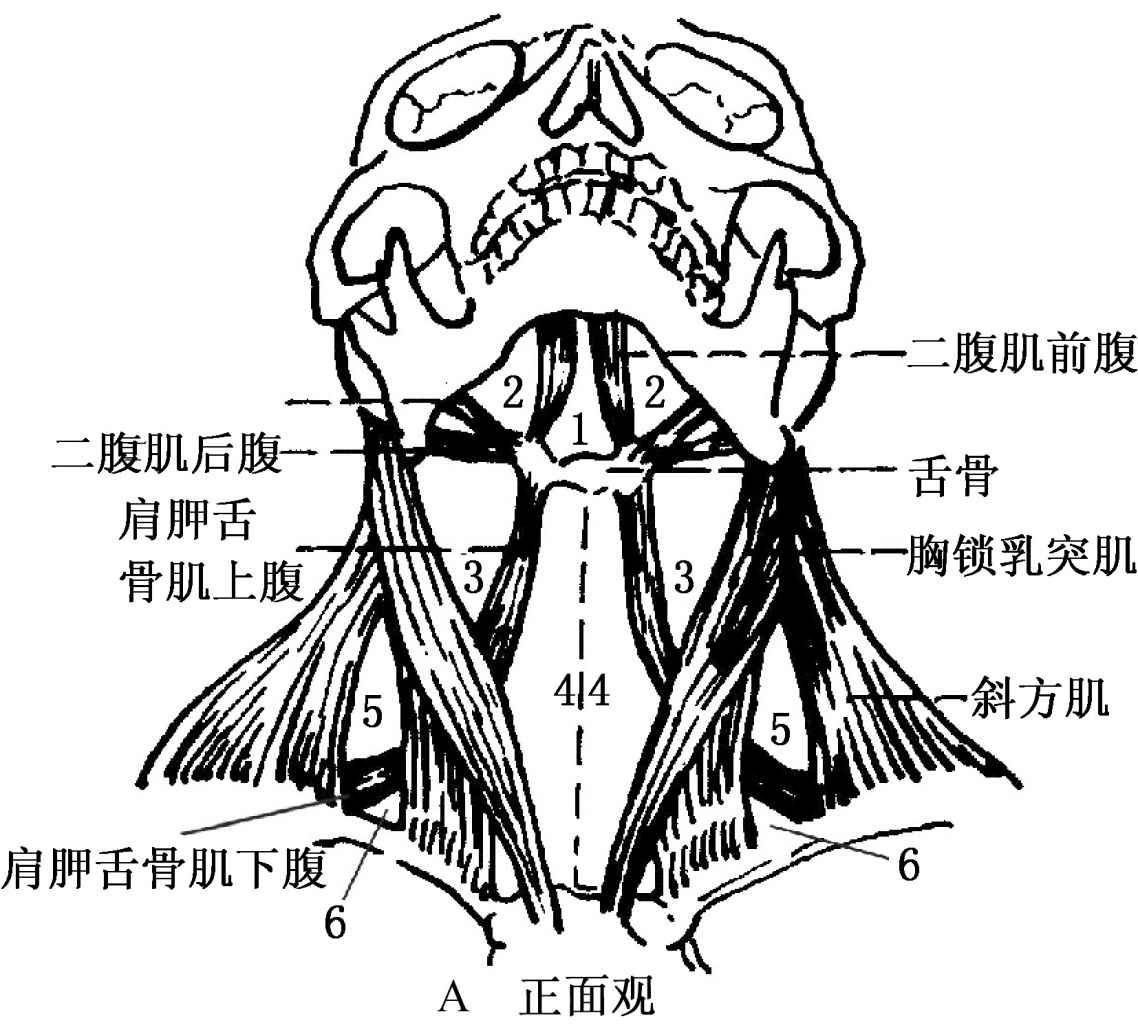
\includegraphics[width=.5\textwidth,height=.5\textheight,keepaspectratio]{./images/Image00166.jpg}
 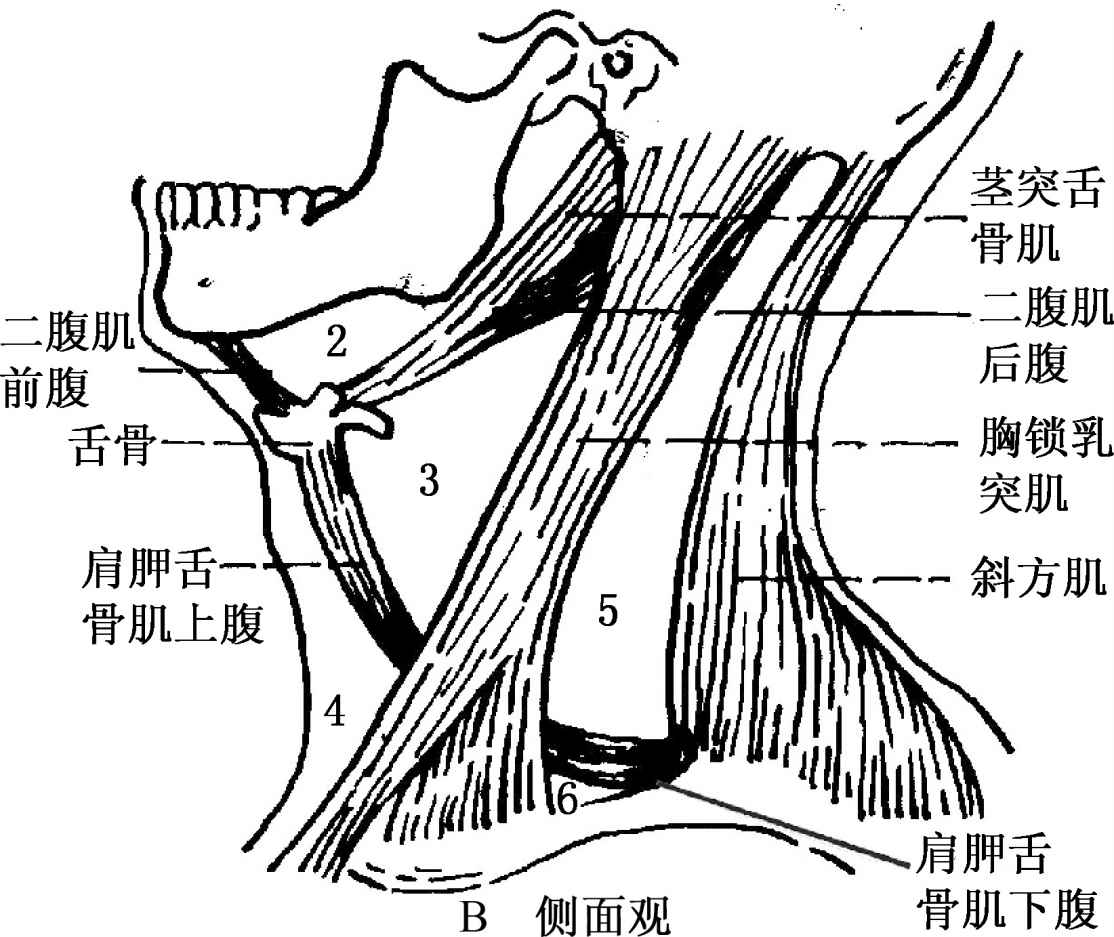
\includegraphics[width=.5\textwidth,height=.5\textheight,keepaspectratio]{./images/Image00167.jpg}
 \captionsetup{justification=centering}
 \caption{颈部分区\\{\small 1.颏下三角;2.颌下三角;3.颈动脉三角;4.肌三角;5.枕三角;6.锁骨上三角}}
 \label{fig8-1}
  \end{figure} 

\subsection{颈部的CT分区}

为叙述方便在CT下通常将颈部分为4个区。

1.脏器区:或称中央区。位于颈部最前面,主要的结构是下咽部、喉部和气管、食管、甲状腺和甲状旁腺。舌骨下带状肌起自喉软骨,止于前上胸壁,是内脏区的前缘。

2.两个外侧区:包括颈动脉间隙、咽后间隙、咽旁间隙等,也包括胸锁乳突肌。在CT轴位像上胸锁乳突肌多位于外侧,其下方是颈动脉鞘。在上颈部,颈内静脉位于颈动脉之后,在中颈部位于颈动脉之外侧,在下颈部位于颈动脉之前。颈动脉分叉大约在舌骨水平。

3.后区:主要是颈椎和肌肉。颈椎被两组肌群包绕。①伸肌群;位于颈椎横突后方;②屈肌群:位于颈椎前方。

\subsection{甲状腺}

甲状腺由两个侧叶及中间的峡部组成。两个侧叶不一定对称。甲状腺位于甲状软骨之下,紧贴第3、第4气管软骨环前方,但下极有时可达第5、第6气管环水平。每叶高约5.0cm,宽约2.5cm,厚约2.0cm;峡部较薄,高约2.0cm。正常腺体侧叶的后方被筋膜(假被膜)形成的甲状腺悬韧带固定在环状软骨下方的气管上,故吞咽时甲状腺可上下移动。甲状腺由颈内脏层筋膜所组成的鞘包绕称为假被膜。甲状腺本身还有一层纤维组织膜称为真被膜,其纤维伸入腺体,将腺体分成小叶。

其血液供应有来自颈外动脉和锁骨下动脉的甲状腺上、下动脉,经甲状腺上、中、下静脉回流。与甲状腺位置关系密切的神经有喉上神经和喉返神经。在甲状腺下极部喉返神经及甲状腺下动脉位于气管食管沟内。

CT表现:腺体常呈楔形或三角形,多边界清楚。含碘平扫密度高于周围以及前方的肌肉组织,一般密度较均匀。增强扫描时腺体强化明显,并可显示供血动脉。

\subsection{甲状旁腺}

甲状旁腺通常有上、下两对,但亦可多于或少于4个,正常为2~5个。直径约1cm。上一对位于甲状腺侧叶近上极部后面内侧;下一对多位于甲状腺下极的后外侧(喉返神经的外侧)、甲状腺下动脉附近。有时甲状旁腺可埋藏于甲状腺实质内,称为迷走甲状旁腺。甲状旁腺无独立的血管系统。正常情况下甲状旁腺在CT图像上不能显示。

\subsection{颈深筋膜的分层}

颈部器官大多呈纵向排列,周围被筋膜及疏松结缔组织包绕,下延至纵隔。颈筋膜有深、浅之分:①颈浅筋膜:在颈部皮下,附着于颈阔肌表面。②颈深筋膜:又分为浅、中、深3层,叙述如下:

1.颈深筋膜浅层:又称为封套筋膜。其上方附着于下颌骨下缘、乳突、上项线和枕外粗隆,下方附着于胸骨柄、锁骨和肩峰。自颈椎棘突开始向前分层包绕斜方肌、胸锁乳突肌和咀嚼肌,然后两侧于颈前中线对接,附着于舌骨后。在舌骨上再分层包绕颌下腺、腮腺,其浅表一层成为腮腺咬肌筋膜,附着于颧弓;深面一层延续成为颊咽筋膜,附着于颅底。在舌骨下则包绕舌骨下肌群。

2.颈深筋膜中层:又称为气管前筋膜或内脏筋膜。位于舌骨下肌群深层,向上附于舌骨、甲状软骨和环状软骨,并包绕颈部脏器(咽、食管、喉、气管、甲状腺和甲状旁腺)形成脏层间隙。包绕甲状腺部分形成其假被膜;向下经胸骨柄后方与纵隔筋膜相连;在气管前方形成气管前筋膜。

3.颈深筋膜深层:又分为翼筋膜和椎前筋膜。翼筋膜位于椎前筋膜前方,向两侧的部分包绕颈总动脉(或颈内动脉)、颈内静脉和迷走神经形成颈动脉鞘(间隙)。椎前筋膜覆盖于椎体、椎前肌和斜角肌表面,自颅底下延至后纵隔与心包膜相连。

\subsection{颈部的间隙}

颈部由颈深筋膜分为多个间隙(图\ref{fig8-2}):①在舌骨上有:咽黏膜间隙、嚼肌间隙、咽旁间隙、腮腺间隙、颈动脉间隙、咽后间隙和椎前间隙等。②在舌骨下有:脏层间隙、颈动脉间隙、咽后间隙、椎前间隙和颈后间隙。

\begin{figure}[!htbp]
 \centering
 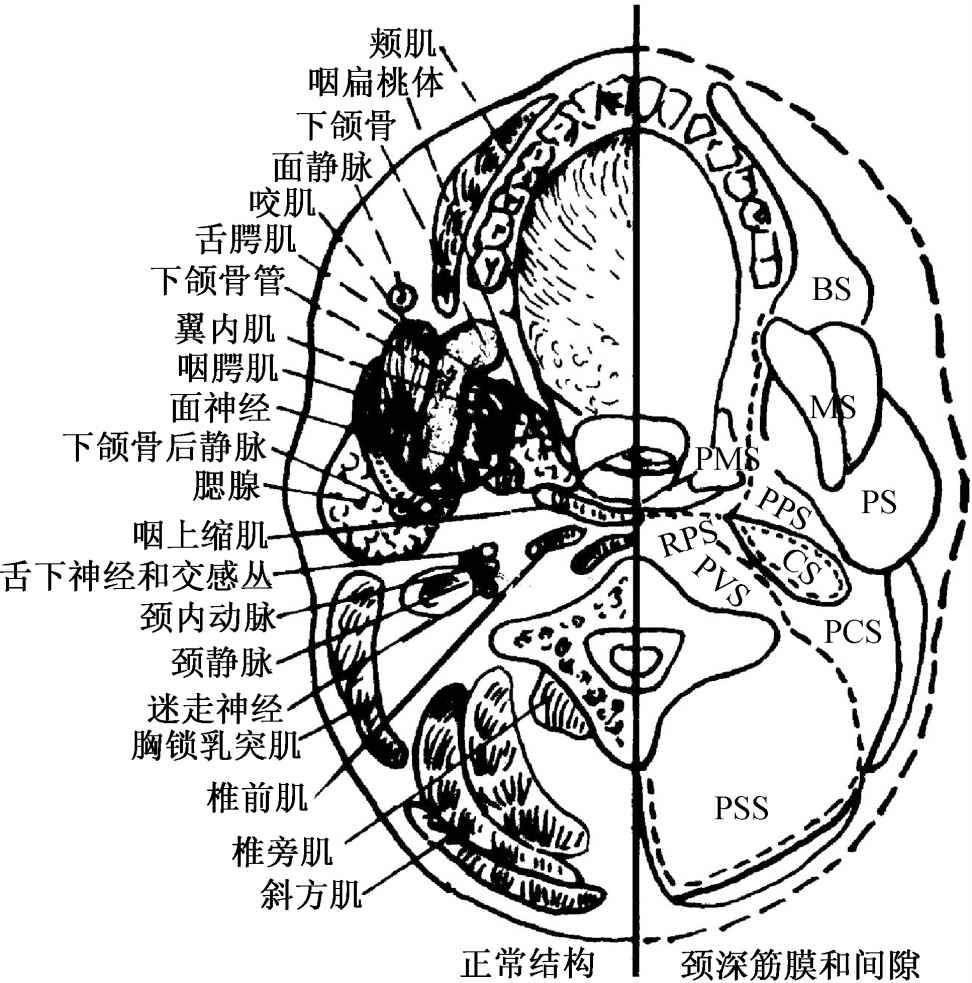
\includegraphics[width=.7\textwidth,height=\textheight,keepaspectratio]{./images/Image00168.jpg}
 \captionsetup{justification=centering}
 \caption{口咽的横断面解剖\\{\small BS颊黏膜间隙;MS嚼肌间隙;PS腮腺间隙;CS颈动脉间隙;PVS椎前间隙;PPS咽旁间隙;PMS咽黏膜间隙;PCS颈后间隙;RPS咽后间隙;PSS椎旁间隙}}
 \label{fig8-2}
  \end{figure} 

有关咽黏膜间隙、嚼肌间隙、咽旁间隙、咽后间隙、腮腺间隙等已在有关章节(第六章第二节)中叙述。

1.颈动脉间隙:又称颈动脉鞘。自颅底向下延伸至主动脉弓。外侧为胸锁乳突肌;内侧为咽后间隙;前方以茎突与咽旁间隙(或称为咽旁间隙的前内部分)分界;后内以颈长肌、前斜角肌与椎旁间隙分界。其内主要含颈动、静脉(在舌骨上包含颈内动、静脉,在舌骨下包含颈总动脉、颈内静脉),颈静脉链淋巴结,Ⅸ~Ⅻ对颅神经及交感神经链。颈静脉链淋巴结位于颈动、静脉的外、前、后方。第Ⅸ~Ⅻ对颅神经及交感神经链在舌骨上区位于血管的内、后方,至舌骨下区第Ⅸ、Ⅺ、Ⅻ对颅神经已分出,只剩下迷走神经走行于颈动、静脉之间稍偏后,交感神经链仍位于血管的内、后方。颈动脉分叉大约在舌骨水平。在舌骨上颈内动脉位于颈内静脉前内。颈外动脉在颈动脉鞘外,位于颈内动脉更前方。在颈中部颈内静脉居颈动脉外侧,在颈下部位于颈动脉前方。一般颈内静脉较颈动脉粗大。双侧颈内静脉可不等大,右侧常较大,尤其在颈下段。

2.椎前间隙:在咽后间隙之后,咽后间隙是位于咽后壁颊咽筋膜(咽缩肌后面覆有颊咽筋膜)与椎前筋膜(椎前肌)之间的潜在间隙。椎前间隙位于椎前筋膜与脊柱之间,下延至后纵隔,此间隙内有头直肌、头长肌(第3颈椎以上)和颈长肌(下达第1~3胸椎水平)统称为椎前肌。双侧椎前肌在颈椎前中线有肌嵴和韧带分隔。横断面CT可显示,一般双侧对称。

3.椎旁间隙:位于颈动脉间隙之后,以前斜角肌和中斜角肌为其前、后界,此间隙通过颈部全长。在第3~5颈椎水平,前斜角肌之前的筋膜深部有膈神经,在第5颈椎至第1胸椎水平,前和中斜角肌间有脊神经臂丛及其分支。

4.气管前间隙:在气管与胸骨甲状肌之间,由颈内筋膜壁层与脏层形成的潜在间隙,向下达前上纵隔。

5.内脏间隙:位于颈内筋膜壁层与脏层之间,自颅底向下经后纵隔至横膈处。其内包含咽、食管、喉、气管、甲状腺、血管及淋巴组织。

\subsection{颈部淋巴结}

1.颈外侧深部淋巴结群:又分为3组,①颈深淋巴结链:沿颈内静脉分布,位于颈动脉鞘内。以舌骨平面和环状软骨为界分为上、中、下三组。颈深淋巴结链的最高部位位于下颌角处,最低部位为Virchow
淋巴结。该淋巴结链接受腮腺、咽后、颌下和颏下等淋巴结引流,形成颈淋巴干,引流入锁骨下静脉或颈内静脉,在左侧进入胸导管,而后进入静脉系统。②脊副淋巴结链:即颈后三角淋巴结链。沿副神经分布,位于颈后三角区内。该淋巴链接受枕部、乳突、头皮、外侧颈部淋巴引流,然后进入颈横淋巴结链。③颈横淋巴结链:又称锁骨上淋巴结链,位于锁骨上区并与锁骨平行,呈水平走向。接受颈后三角淋巴结链、颈深淋巴结链、锁骨上淋巴结、前上胸壁和颈前外侧皮肤的引流,最后进入静脉系统。

2.颈前淋巴结链:分为两组:①浅组:为颈前静脉组,沿颈外静脉走行,位于颈部浅层的筋膜间隙中,引流颈前部皮肤和肌肉的淋巴。②深组:为食管旁淋巴链,位于气管旁、甲状腺后方的气管食管沟内。

3.颌下-颏下淋巴结链:①颌下组:位于颌下三角的后外侧,邻近颌下腺,接受前半面部、皮肤、口腔等处的淋巴引流。②颏下组:位于颏下三角、二腹肌前支的前方。接受颏、唇、颊、口底、舌的淋巴引流,然后引流入颌下组,最后进入颈深上淋巴结组。

4.腮腺组:分为腺内组和腺外组,均位于腮腺间隙内。主要引流前额部和颞部皮肤、后颊、龈和颊黏膜淋巴,最后进入颈深淋巴结链。

5.咽后组:分为两组:①内侧组:靠近中线;②外侧组:位于咽后间隙的外侧、颈内动脉的内侧、椎前肌肉的前方。两组均接受鼻咽、口咽的淋巴引流,然后进入高位颈深淋巴结链。

颈部正常淋巴结直径一般在0.3~1.0cm,>1.5cm为异常。咽后组一般<0.7cm,>1.0cm为异常。

\section{先天性囊性病变}

\subsection{甲状舌管囊肿}

本病是儿童及成人最常见的颈部囊性病变。可在舌根至胸骨切迹之间沿正中线的任何部位形成囊肿。舌骨上方占65%,舌骨下方占20%,舌骨前方占15%。

\textbf{【病因】}
甲状舌管始于甲状腺原基,胚胎第4周原基组织开始下降,并向前发展成甲状舌管或甲状腺囊,此囊上止于舌盲孔,向下发育成甲状腺。如果第10周甲状舌管导管退化不全、没有消失,以后则有可能发展成甲状舌管囊肿,如舌甲管部分开放则形成瘘管。

\textbf{【临床表现】}
儿童期症状不明显,多数到青少年甚至中年才发现。囊肿较小时一般无自觉症状,较大时可有咽部压迫感、异物感。颈中线前方可扪及质地柔软或较硬的软组织肿块。合并感染时可有疼痛或穿破形成瘘管。本病应首先B超检查,因为它有利于鉴别囊实性。

\textbf{【CT表现】}
表现为舌骨上下区域的圆形低密度或等密度灶,边缘清楚光滑。囊液CT值与蛋白含量有关,约20Hu。有时可偏于一侧。舌甲囊肿可在舌骨外面、颈部皮下或喉外生长,也可部分骑跨舌骨甚至甲状软骨进入喉咽或喉腔,致甲状软骨板分离或压迫性骨质吸收。较小者需以2mm层厚扫描,以免因部分容积效应而误诊。增强扫描囊壁可明显强化。囊肿后缘有一柄状突起,伸入舌会厌韧带与甲状软骨后,为扩张的甲状舌管,其密度与囊肿类似,为本病的特征。继发感染,囊壁增厚,边缘模糊。如囊壁局部增厚、毛糙或囊壁局限软组织突起,应警惕恶变可能。

\textbf{【鉴别诊断】}
①腮裂囊肿:如甲状舌管囊肿偏离中线,应注意与鳃裂囊肿相鉴别。后者多位于下颌角后方,颌下腺与胸锁乳突肌前缘之间,尤其位于颈内、外动脉之间为特征性位置。②表皮样囊肿:前正中区附近表皮样囊肿多呈负值,有助于鉴别。此外,腮裂囊肿和表皮样囊肿不随吞咽而上下移动。

\subsection{鳃裂囊肿}

本病是一种颈部先天性囊性病变。

\textbf{【病因病理】}
胚胎发育至第5周有5对腮弓。每对腮弓的内胚层形成腮囊,外胚层形成腮沟。如腮囊和腮沟发育异常,未被吸收,可发生囊肿、窦道和瘘管。第二腮裂囊肿是第二常见的先天性颈部囊性肿物,约占腮裂囊肿的90%~95%;第一腮裂囊肿占5%~8%,第三、第四腮裂囊肿约占1%。来自腮沟的囊壁衬有鳞状上皮;来自腮囊的衬有呼吸道上皮,但反复炎症发作后可演变为鳞状上皮。腮裂囊肿很少恶变。

\textbf{【临床表现】}
多见于11~50岁之间,以30岁左右多见。主要表现为腮腺或外耳道周围肿物。常无明显症状,较大者可感咽部不适、吞咽有异物感。如伴有瘘管或反复感染,常在颈部胸锁乳突肌前有瘘口、溢脓。

\textbf{【CT表现】}
囊肿呈类圆形均质低密度区,平扫CT值在20Hu左右。有完整光滑的薄壁。囊腔大小不一。增强扫描囊壁有强化。如囊肿继发感染,囊壁可增厚,边缘不光滑,囊内容物CT值略增大。第二腮裂囊肿位于下颌角后方近颌下腺区,致胸锁乳突肌后移,颈动、静脉向后内移位(图\ref{fig8-3})。有时囊肿位于颈内和颈外动脉之间,这是其特征性位置。不典型时可位于咽旁区,表现为咽旁间隙肿物,可被误诊为腮腺深叶肿物。若继发感染,并有化脓性淋巴结增大可能被误诊为恶性肿瘤。

\begin{figure}[!htbp]
 \centering
 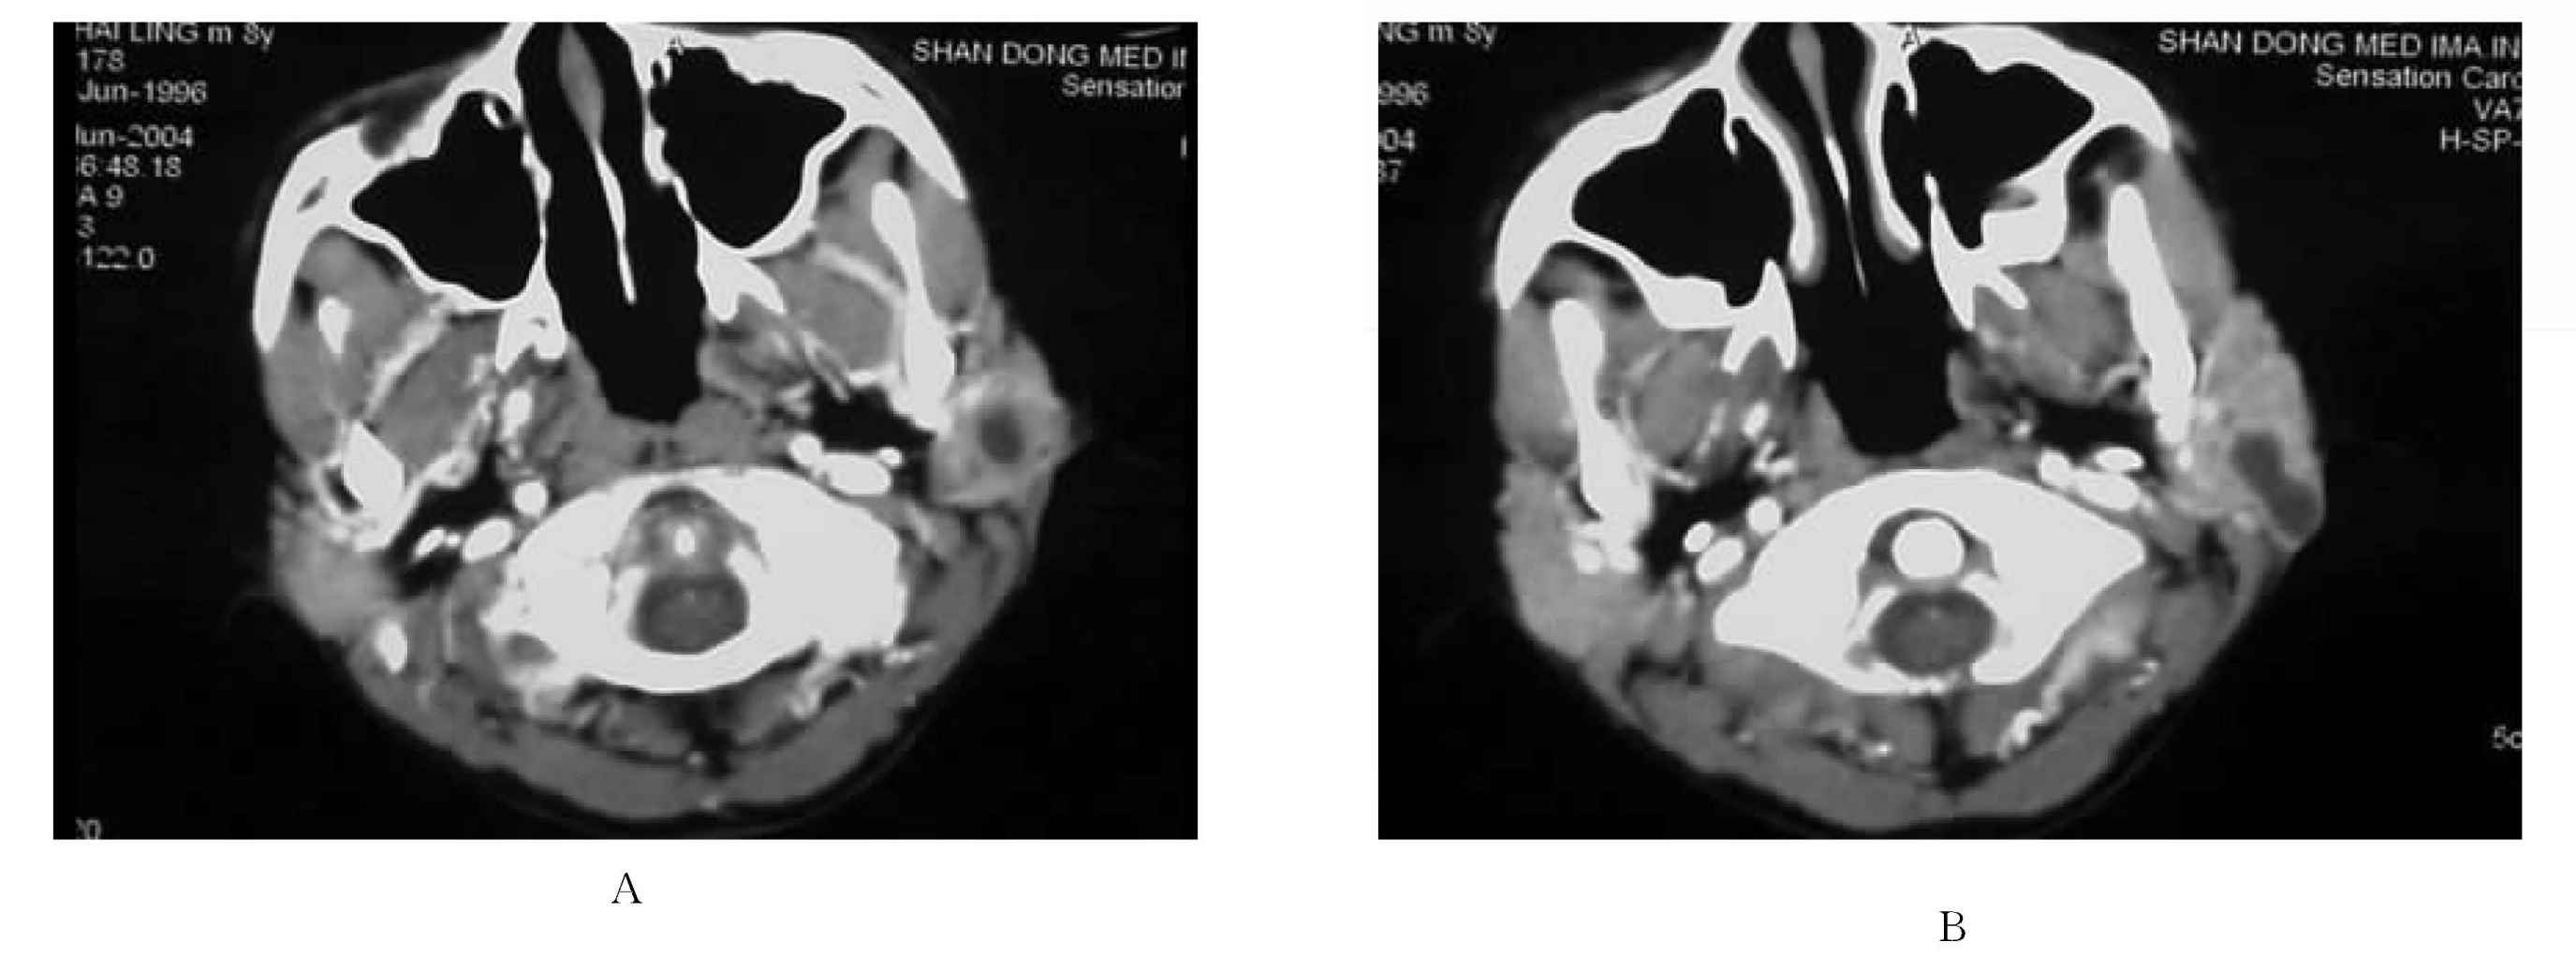
\includegraphics[width=.7\textwidth,height=\textheight,keepaspectratio]{./images/Image00169.jpg}
 \captionsetup{justification=centering}
 \caption{左侧先天性腮裂囊肿(瘘)\\{\small 左侧下颌角后方有水样密度灶,壁较厚(与感染有关,患者局部有瘘管)}}
 \label{fig8-3}
  \end{figure} 

\textbf{【鉴别诊断】}
本病需注意与神经源性肿瘤坏死囊变、颈部脓肿、颌下腺囊肿、囊性淋巴管瘤、坏死性转移瘤或炎症性淋巴结肿大鉴别。

\subsection{颈部淋巴管瘤}

\textbf{【病理】}
淋巴管瘤的病理改变是淋巴管扩张、增生和结构紊乱。可分为毛细淋巴管瘤、海绵状淋巴管瘤和囊样水瘤。头颈部以囊样水瘤最为常见,呈多囊状。囊壁甚薄,内含黄色淋巴液。

\textbf{【临床表现】}
多见于婴幼儿,2岁以内者占80%。颈侧部软性包块、无痛,有波动感,不易被压缩。生长缓慢,易并发感染和出血。

\textbf{【CT表现】}
常位于颈侧部的颈后三角区(75%)。①呈囊性病变,多囊或单囊,以多囊多见,囊内可有分隔,可广泛波及颈深部至皮下,易沿组织间隙生长是其特点;②呈均匀水样密度,囊内易有出血而使平扫密度增高或出现囊内液-液平面;③囊壁可轻度强化;④囊样水瘤可自行消退,但病变部位越深在、越复杂,复发可能性越大,抽吸还可能导致液体的迅速重新积聚。

\textbf{【鉴别诊断】}
腮裂囊肿与淋巴管瘤的区别主要在于前者单个多见,少有出血;而淋巴管瘤常多囊发生或囊内出现多个分隔状改变。

\subsection{颈部胸腺囊肿}

\textbf{【病因】}
原始胸腺源于第三咽囊,于胚胎第6周形成,第7周与咽囊的连接分离,第8周其始基在中线融合并贴于心包,在第12周胸腺组织达上纵隔。如退化不全可发生囊肿。胸腺囊肿可发生于自下颌角到纵隔之间的任何部位且与颈动脉鞘密切相连。国外有报道68%位于左侧,25%位于右侧,7%位于中央。

\textbf{【临床表现】}
本病3~8岁者占65%,男性是女性的3倍。颈部可触及软性包块,无其他症状。

\textbf{【CT表现】}
呈单囊或多囊性病变。边缘光滑锐利,病变至少有部分位于颈动脉鞘内。囊内密度因含蛋白的高低及是否出血而高低不一。

\subsection{颈部囊性病变的鉴别诊断}

颈部囊性病灶的发生部位是进行鉴别诊断的关键。

1.多数甲状舌管囊肿、皮样囊肿、喉囊肿发生于颈中线。甲状舌管囊肿与舌骨关系密切,特别是当囊肿部分延伸至舌骨后时更有意义。皮样囊肿也会发生于中线舌骨周围,但以舌下间隙更常见,且多含有脂肪有助于鉴别。

2.腮裂囊肿、淋巴管瘤和胸腺囊肿多发生于颈外侧。腮裂囊肿常位于上颈部的胸锁乳突肌前缘。而淋巴管瘤75%位于颈后三角区,呈分叶状互不相通的多囊状,向周围组织间隙侵入是其特点。颈部胸腺囊肿至少有部分位于颈动脉鞘内有助于鉴别。

3.颈部炎性淋巴结(包括结核)可见囊变,但常为多发。甲状腺增生可合并部分囊变,但同时可见甲状腺病变的其他表现。

此外,还应注意与囊变的神经鞘瘤相鉴别,神经鞘瘤囊变其壁多较厚,可有厚的间隔;但薄壁的完全囊变的神经鞘瘤不易诊断和鉴别。

\section{颈动脉间隙及其他颈外侧区病变}

\subsection{概述}

\subsubsection{颈部软组织肿瘤的分类}

国内有学者将颈部软组织肿瘤分为6类:①神经源性肿瘤;②涎腺肿瘤;③脉管性肿瘤;④淋巴结病变;⑤脂肪性肿瘤;⑥其他。其中颈部外周神经源性肿瘤(特别是神经鞘瘤)是颈部原发性软组织肿瘤中常见的一种。

\subsubsection{颈动脉间隙、颈后区病变}

1.颈动脉间隙病变:主要有颈动脉体瘤、颈神经鞘瘤或神经纤维瘤、颈动脉瘤以及恶性淋巴瘤或淋巴结转移瘤。

2.颈后区病变:比较少见,多与颈椎和神经组织有关,另外来源于间充质。如颈椎本身的结核及颈后区脓肿;动脉瘤样骨囊肿和骨母细胞瘤多位于颈椎横突和椎弓等;神经源性肿瘤可位于椎管内外。

\subsubsection{颈外侧区恶性肿瘤}

主要是淋巴结转移瘤,一般认为直径>1.5cm有意义,<1.0cm为阴性。鳞癌的淋巴结转移瘤易发生中心坏死。淋巴瘤是最常见的原发性颈部恶性肿瘤。儿童常见的恶性肿瘤是横纹肌肉瘤和纤维肉瘤,其他还有恶性纤维组织细胞瘤、血管外皮瘤等。CT可显示这些肿瘤及其浸润生长的特点,但确诊还需病理组织活检。

\subsubsection{}

\begin{table}[htbp]
\centering
\caption{颈部囊性、环形和实质性强化肿块病变}
\label{tab8-1}
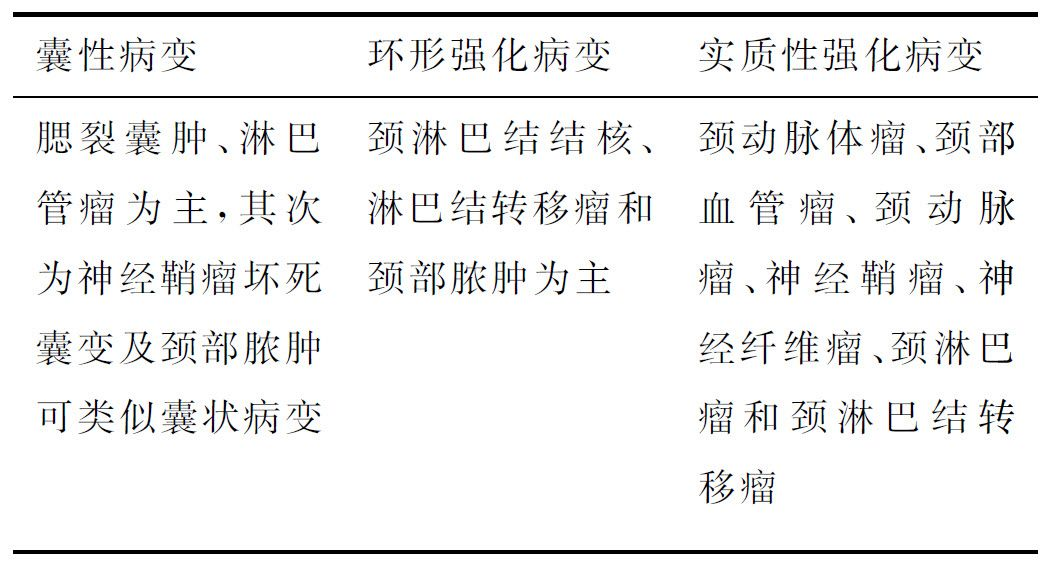
\includegraphics[width=\textwidth,height=\textheight,keepaspectratio]{./images/Image00170.jpg}
\end{table}

\subsection{颈动脉体瘤}

副神经节来源于神经嵴的细胞,这些细胞在胚胎发育过程中,经迁移分散于身体各处,如肾上腺、头、颈、纵隔、腹膜后等。头颈部副节瘤均无分泌功能。头颈部副节瘤以颈动脉体瘤最常见,其次是颈静脉球瘤,眶内睫状体神经节瘤、喉内起源和喉返神经者最少见。

颈动脉体瘤亦称非嗜铬性副神经节瘤,是化学感受器瘤的一种,为少见的颈部肿瘤。颈动脉体绝大多数位于颈总动脉分叉处,少数位于颈部其他大动脉周围。颈动脉体大小约0.5~0.8mm,呈卵圆形,在胎儿期已渐增大,至青春期后渐萎缩。

\textbf{【病理】}
颈动脉体瘤质地中等、有丰富的滋养血管。显微镜下细胞呈巢形围绕血管纤维隔排列,组织学检查很难确定良恶性。淋巴或远处转移及切除后复发是恶性的主要特征。恶性者国内报道不超过5%。

\textbf{【临床表现】}
多发于青春期,女性多于男性。常表现为颈部无痛性肿物,可压缩,与皮肤无粘连。多位于下颌角的下方和胸锁乳突肌的前侧。较大时可压迫颈内、外动脉致晕厥、耳鸣、视力模糊等症状。颈交感神经受压时可出现Horner征。

\textbf{【CT表现】}
平扫于颈内、外动脉分叉处或附近可见椭圆形结节或肿块,密度均匀,边缘清楚。增强后肿瘤显著强化,CT值可达90~130Hu。有的瘤体内可见多数高密度强化的条状分隔,为瘤体内血管纤维间隔强化而成。其时间-密度曲线峰值与颈内动脉峰值相比幅度稍小、出现稍晚为其特征性征象。肿瘤可使颈内、外动脉之间的距离加大,血管受压变细以及产生不同程度的移位,具有重要的诊断价值。

\subsection{颈部神经鞘瘤和神经纤维瘤}

颈部神经源性肿瘤可分为神经鞘瘤和神经纤维瘤。前者起源于神经鞘细胞(雪旺细胞),后者起源于神经鞘的神经纤维母细胞。在颈部多数是神经鞘瘤,神经纤维瘤少见。可发生于颈部的任何神经如迷走、舌下、交感、膈、颈丛及臂丛神经等,但以来自颈交感神经、迷走神经者为最多,故常见于颈动脉鞘区。

\textbf{【病理】}

1.神经鞘瘤:大多由梭形细胞组成。有包膜,常有坏死囊变。病理主要有Antoni
A区和Antoni B 区组成。Antoni A区细胞排列紧密,Antoni
B区细胞少,排列稀疏呈网格状;细胞间有黏液变性和高脂质。各种神经鞘瘤两者的比例不同,可以从完全的Antoni
A 区,逐渐过渡到两者交错,甚至完全被Antoni
B区所占据。更有甚者可完全退变形成一个大囊。

2.神经纤维瘤:含有全部神经纤维组织成分,也可包含雪旺细胞或富脂质细胞,无包膜。神经常穿越在肿瘤之中而不受推移。常为实性,因肿瘤内含有各种成分,故亦可有坏死、囊变,但少见。

\textbf{【临床表现】}
多发生于30~40岁成人,男性多见。一般病程较长,除颈部肿块外,多无其他症状。肿块边缘清,表面光滑,呈囊性或较软的多为神经鞘瘤。其他压迫症状基本同颈动脉体瘤。

\textbf{【影像学表现的病理基础】}

1.神经鞘瘤:如以Antoni A区为主时则表现为均质高密度,以Antoni
B区为主时呈均质低密度肿块。如二者接近等同而混合存在时,即呈斑驳不均质密度肿块,并呈斑驳样强化,具有特征性。总之,神经鞘瘤因含有黏液和高脂质而密度常低于肌肉。增强程度多由平扫的20~50Hu增至60~70Hu,少数可增至90~98Hu。

2.神经纤维瘤:常呈实性,少有囊变,密度不均,因含脂质细胞而密度常低于肌肉。理论上讲应高于神经鞘瘤。

\textbf{【CT表现】}
肿瘤呈圆形或椭圆形边缘清楚的软组织肿块,就诊时肿瘤多>3cm。肿瘤呈软组织密度(但常低于肌肉),肿瘤较小者密度均匀,较大的神经鞘瘤易出现坏死、囊变,甚至偶可钙化(图\ref{fig8-4})。增强后两者均呈轻度强化,坏死区不强化。

\begin{figure}[!htbp]
 \centering
 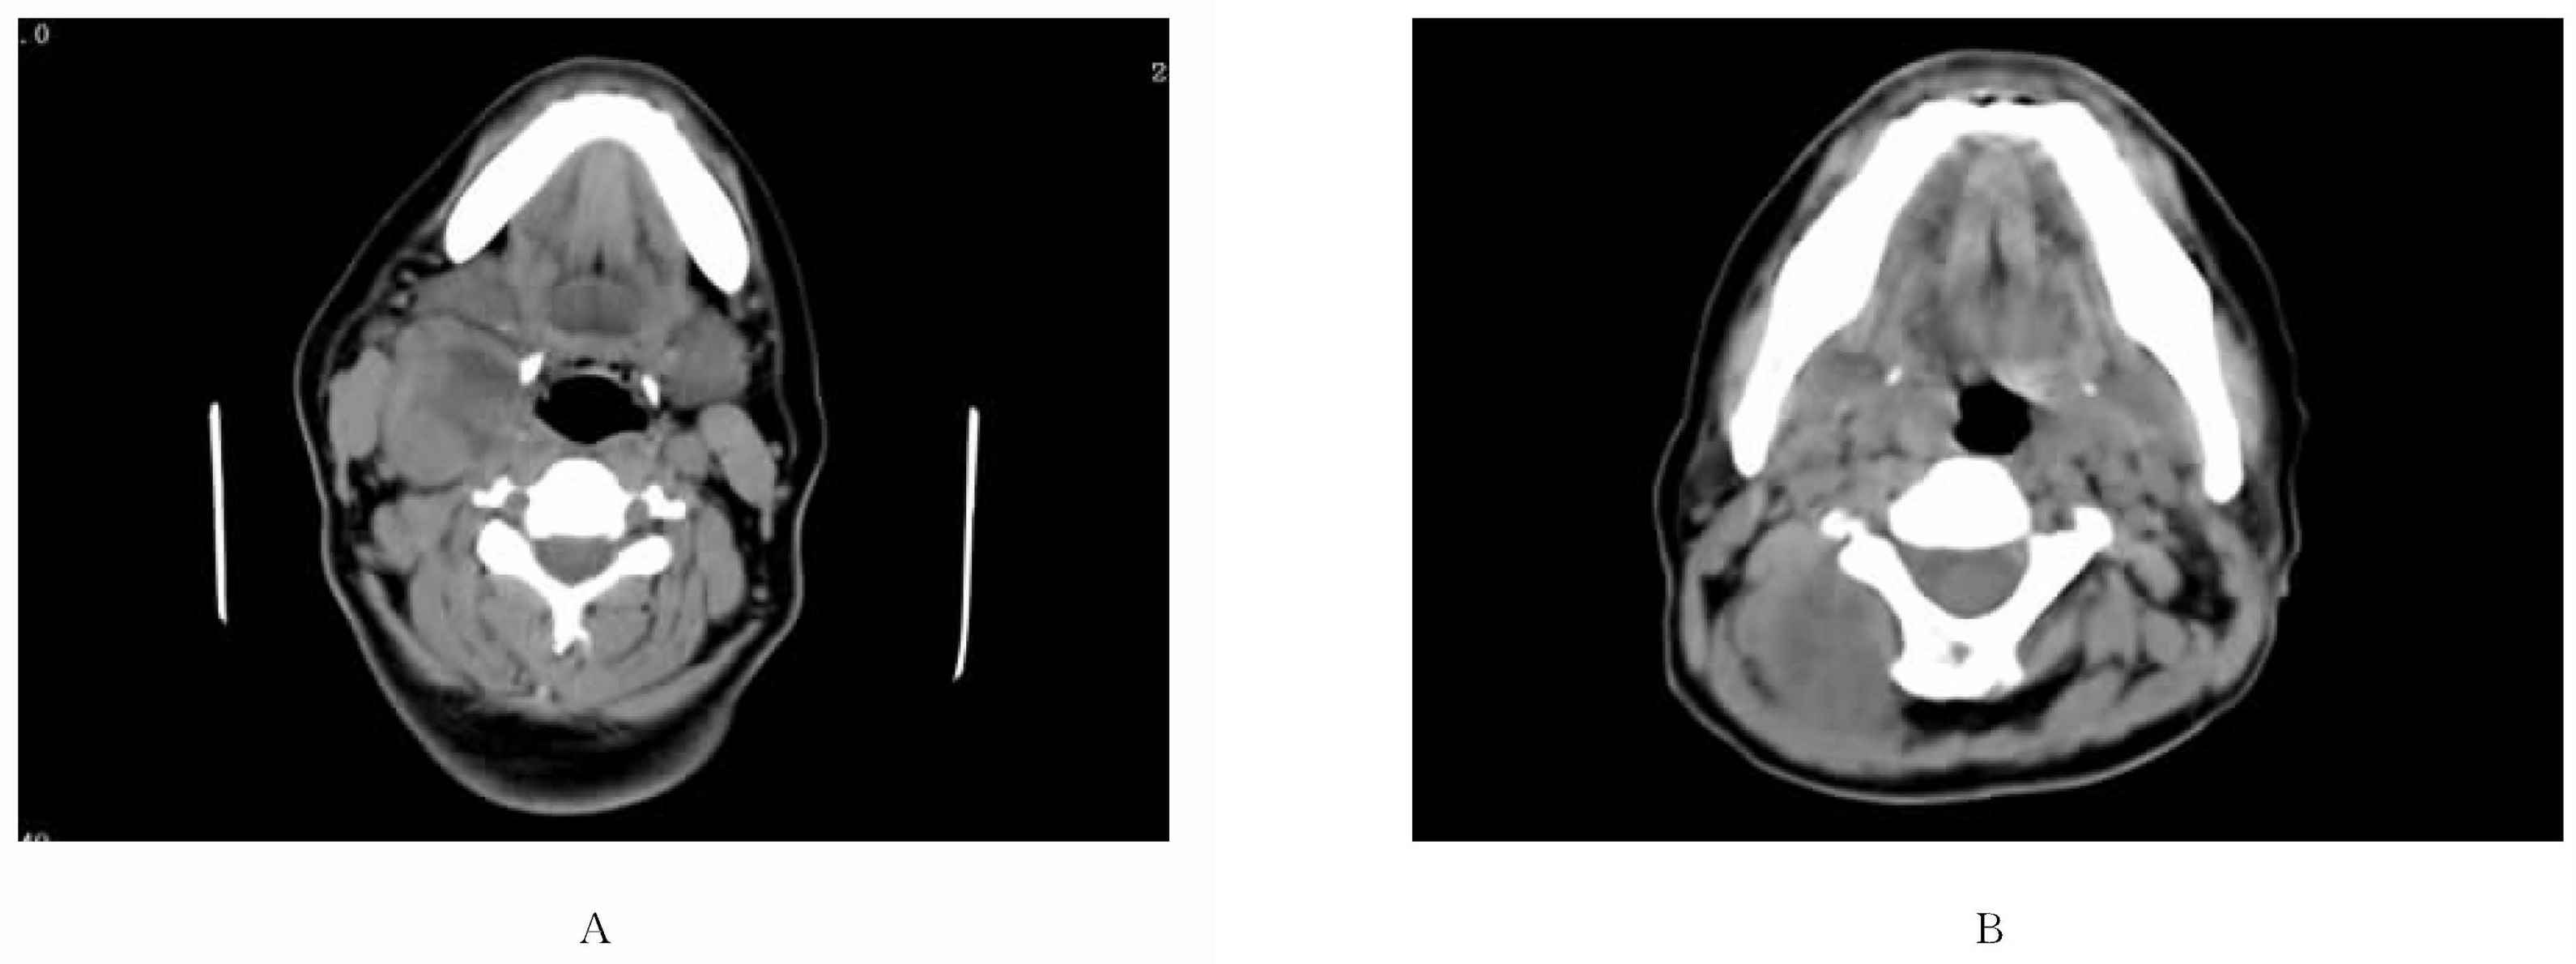
\includegraphics[width=.7\textwidth,height=\textheight,keepaspectratio]{./images/Image00171.jpg}
 \captionsetup{justification=centering}
 \caption{颈部神经鞘瘤\\{\small A.右侧颈部近颈动脉鞘区有软组织肿块,界限清晰,其内有不规则低密度坏死区;B.右侧颈部椎旁有软组织肿块,界限清晰,其内有明显低密度坏死囊变区}}
 \label{fig8-4}
  \end{figure} 

瘤内出现坏死尤其是大的坏死区是神经鞘瘤有别于神经纤维瘤的重要CT表现;斑驳样不均质低密度肿块或斑驳样强化亦为神经鞘瘤较特征性表现。恶性神经源性肿瘤密度不一,无特征性。颈动脉间隙神经源性肿瘤多为单发。因位于颈动、静脉的内侧或后方,故推压血管向外侧或前方移位,在舌骨上区还推压茎突前移。肿块向前方推移颈内外动脉,颈内外动脉分叉可扩大,但不如颈动脉体瘤常见和明显。

颈部神经源性肿瘤有特定的解剖部位,为诊断提供了有利条件。如颅神经肿瘤位于颈静脉窝、咽旁间隙、颈动脉间隙,上交感神经链肿瘤位于颈动脉后方、颈长肌前方;脊神经根肿瘤位于椎旁间隙和椎间孔处;臂丛神经根肿瘤位于斜角肌间隙;膈神经肿瘤在前斜肌前方等。根据这些窝或孔有无扩大和骨质改变、间隙有无移位或消失,颈动、静脉和肌肉移位方向等可以推测肿瘤的起源。如:①椎间孔扩大为来自颈神经根的肿瘤;②颈动、静脉后移多为来自舌下神经的肿瘤(舌下神经者可使舌下神经管扩大,临床出现声嘶、吞咽障碍等症状);③颈动、静脉前移多为来自迷走神经的肿瘤,亦有人认为颈动、静脉分离为迷走神经肿瘤的特征性表现;④颈动、静脉前移同时伴有颈长肌后移则为来自交感神经链的肿瘤;⑤前斜角肌后移则为来自膈神经根的肿瘤;⑥斜角肌间隙消失则为来自臂丛神经根的肿瘤。

\subsection{颈动脉瘤}

本病为颈动脉壁局部薄弱扩张而形成,呈囊状或梭形。

\textbf{【临床表现】}
多见于中老年。生长速度慢,呈囊性或较软的肿块,压迫后可缩小,有波动感。

\textbf{【CT 表现】}
①平扫为类圆形软组织肿块(血液密度),密度均匀,边缘清楚,不分叶;②增强扫描呈高度强化,强化程度与同层颈动脉一致。

\textbf{【鉴别诊断】}
①颈动脉体瘤:亦可呈均匀显著强化,但其好发于颈内、外动脉分叉处,并致其间距增宽为其特征;且动脉瘤的强化与其他动脉强化一致。②神经源性肿瘤:轻度强化,且神经鞘瘤易坏死、囊变有助于与颈动脉瘤及颈动脉体瘤相鉴别。

\subsection{颈部血管瘤}

本病多为海绵状血管瘤。小儿较多见。病理上由许多海绵状血窦构成。

\textbf{【临床表现】} 肿块生长速度慢,较柔软,界限欠清。多无其他症状。

\textbf{【CT表现】}
平扫为软组织肿块,边缘清楚,可呈分叶状;如有钙化尤其静脉石样钙化有特征性。增强扫描高度强化,可呈多灶性结节状或迂曲的管状强化,且强化持续时间长。但我们曾见1例,含有一枚静脉石样钙化灶,仅轻度强化。

\textbf{【鉴别诊断】}
①颈动脉瘤:整个瘤体呈明显均匀强化,且与同层动脉一致,无分叶;而血管瘤呈多结节状显著强化,可有分叶,含有静脉石等有助于鉴别。②先天性颈静脉扩张:颈静脉壁先天发育缺陷或颈内静脉瓣关闭功能不全所致,结合增强扫描与其不难鉴别。

\subsection{颈淋巴结转移瘤}

颈部恶性肿瘤中20%为原发性,80%为转移性。其中转移瘤80%来自头颈部,20%来自胸腹部恶性肿瘤。

\textbf{【病因病理】}
颈部淋巴结转移多为鳞状细胞癌,主要来自口腔、鼻窦、喉及咽部,腺癌多来自甲状腺、涎腺和鼻腔;主要分布在颈内静脉区、胸锁乳突肌周围淋巴结。原发于胸腹腔的转移瘤以腺癌居多,多来自乳腺、胃肠道等,常分布在锁骨上区淋巴结。

\textbf{【临床表现】}
多在颈外侧部及锁骨上出现肿大淋巴结,其特点是质硬、多发、结节较固定、压痛。

\textbf{【CT表现】}
颈动脉鞘区及其周围有多个大小不等的软组织密度结节,有些结节融合成块,最大的淋巴结常>3cm(图\ref{fig8-5})。可侵犯颈内静脉(出现瘤栓)和甲状腺等。增强扫描病灶有轻度强化,密度可均匀或略不均匀。有的患者病灶边缘可出现环形强化,其中央部可以是坏死,也可以是实质性肿瘤。所以,如环形强化所包绕的中央部有强化常提示为转移瘤。如坏死的结节与无坏死的结节共存时,对本病的诊断有重要价值。

\begin{figure}[!htbp]
 \centering
 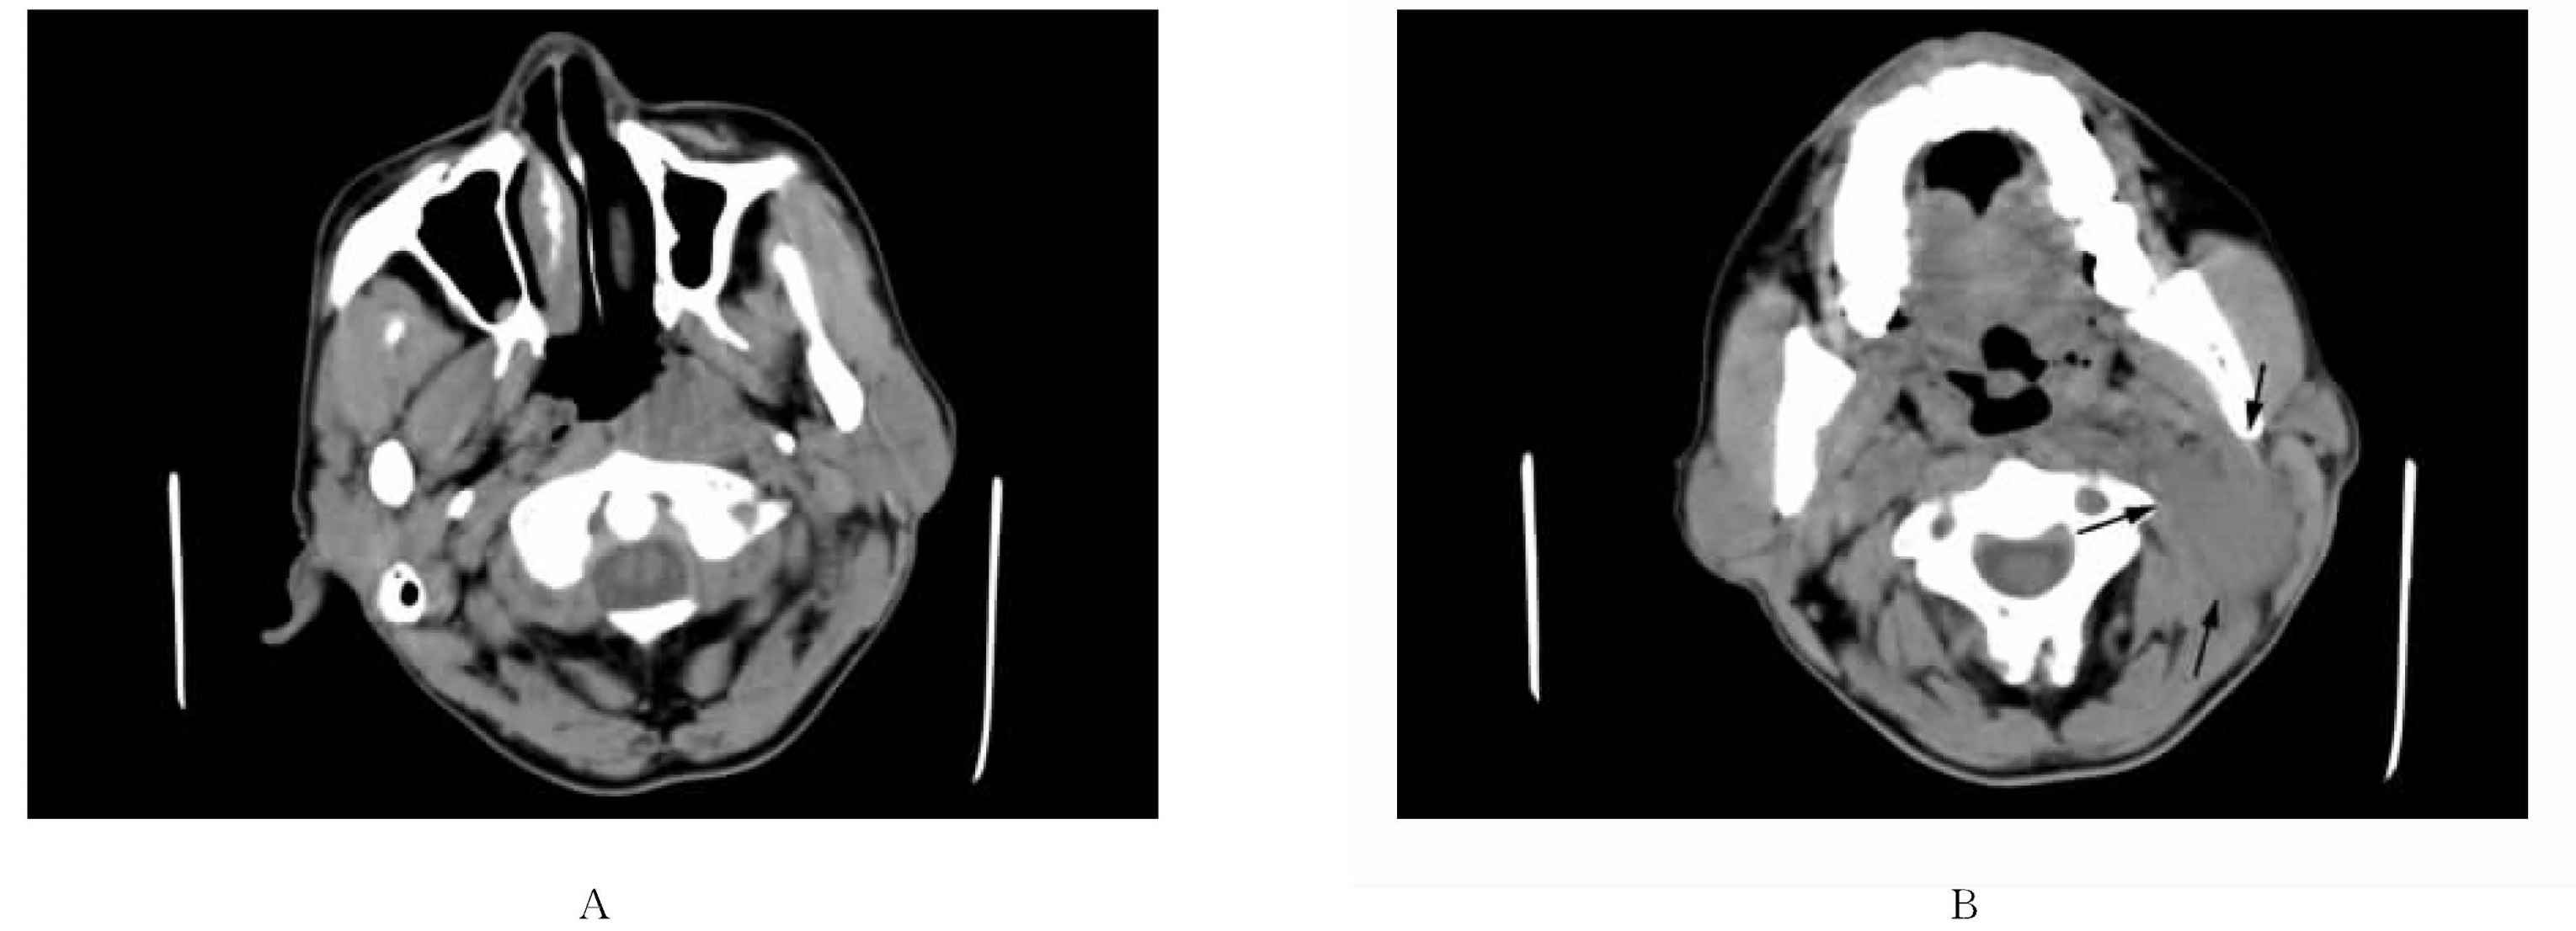
\includegraphics[width=.7\textwidth,height=\textheight,keepaspectratio]{./images/Image00172.jpg}
 \captionsetup{justification=centering}
 \caption{鼻咽癌并左侧颈部淋巴结转移瘤\\{\small A.左侧鼻咽部有软组织肿块,咽隐窝消失;B.左侧颈部胸锁乳突肌下有肿大淋巴结}}
 \label{fig8-5}
  \end{figure} 

淋巴结转移的CT诊断标准:综合国内外有关文献,淋巴结最大横径在颌下、颏下≥10mm,其他区域≥8mm,气管食管沟≥5mm,即视为转移。正常淋巴结趋向于槟榔形或豆状,而转移淋巴结则呈圆形和球形。

在临床工作中遇到原发灶不明时:①如淋巴结不均匀环状强化(偶可均匀环状强化),其内有小低密度区或不规则斑片状低密度区,应首先考虑头颈部鳞癌的可能;②如伴有咽后组淋巴结和(或)颈后三角区淋巴结增大时,在除外淋巴瘤的基础上,应首先考虑鼻咽癌;③如淋巴结边缘清楚、有明显强化,密度与正常甲状腺或甲状腺肿瘤一致,可考虑甲状腺癌;尤其伴有气管食管沟或上纵隔淋巴结肿大时,则可能性更大;④当颈部淋巴结内有囊性变,囊壁内有乳头状结节及细颗粒状钙化,无论甲状腺是否有肿物,都要考虑甲状腺癌(特别是乳头状癌)的可能;⑤此外,腮腺恶性肿瘤的转移淋巴结边缘常呈轻至中度环状强化,中央低密度;还应注意排除胸部(肺、乳腺、食管等),甚至腹部等原发肿瘤转移的可能。

\subsection{颈淋巴瘤}

颈淋巴瘤包括非何杰金和何杰金淋巴瘤。

\textbf{【临床表现】}
青壮年多见,以双侧颈部多发结节或肿块为主诉。患者可同时有发热、乏力、消瘦等症状。腋窝、腹股沟淋巴结亦可增大,肝、脾肿大可能是常见的体征。

\textbf{【CT表现】}
可侵犯颈部任何区域的淋巴结。表现为双侧或一侧颈外侧部有多个增大淋巴结,呈均匀软组织密度,边缘清楚。融合较大的病灶可达5cm以上。增强后瘤灶轻中度均匀强化。坏死和钙化少见。结节少有坏死是其与颈淋巴结转移瘤的重要鉴别点。

\subsection{颈淋巴结结核}

颈淋巴结结核既可发生于颈外侧部的颈深淋巴结,也可发生于颈浅淋巴结。肿大的淋巴结常多发,以一侧多见。

\textbf{【病理】}
分为4个阶段:①淋巴组织增生,形成结节或肉芽肿;②淋巴结内干酪或坏死液化;③淋巴结包膜破坏,互相融合且合并淋巴结周围炎;④干酪物质穿破至周围软组织形成冷脓肿或窦道。就诊时病理多已有干酪性变。

\textbf{【临床表现】}
多见于中青年女性,多以颈部结节就诊,无痛、可移动。实验室检查血沉可增快。

\textbf{【CT表现】}
病灶多位于中下颈部及颈后三角区。平扫见颈部胸锁乳头肌后方或前方、锁骨上下区有多个软组织密度结节,边缘较清楚且边缘密度较中央高。增强后多数结节呈边缘性环形强化、中央无强化(文献报道90.6%有此表现),且可见多个环形强化灶融合在一起。最大的淋巴结一般<2cm。环形强化常提示干酪性结核的存在,有一定特征,这是由于患者就诊时病灶多已发生干酪样变所致。结核性淋巴结炎易融合成团,与邻近肌肉粘连,常引起皮下脂肪层呈渔网状改变,局部皮肤增厚或破溃。

CT增强表现可分为3型:Ⅰ型:均匀等密度强化;Ⅱ型:薄环形周边强化;Ⅲ型:不均质强化。各种类型可同时存在。

国内有学者认为其影像学特点为“三多”:即病变数目多(常融合成团)、侵犯区域多和多种病理改变同时存在。

总之,中青年女性患者有颈部无痛性肿物时,由上述影像学表现者,应首先考虑淋巴结核。

\textbf{【鉴别诊断】}

1.颈淋巴结转移瘤:颈淋巴结结核与颈淋巴结转移瘤症状相近,后者可有原发肿瘤史。其CT表现可有以下不同:①颈淋巴结结核以环形强化多见,常多个聚集于一处呈花环状,淋巴结最大径常<2cm;而淋巴结转移瘤少有环形强化,如有环形强化也常多个发生,且其范围较淋巴结结核广泛,可双侧,淋巴结常>2cm。结核性淋巴结炎易融合成团,与邻近肌肉粘连,常引起皮下脂肪层呈渔网状改变,局部皮肤增厚或破溃,此征象少见于转移瘤和淋巴瘤。②前者发展到环形强化时,中央无强化;后者有时环形强化之中央可有一定程度的强化,而提示为淋巴结转移瘤。③如增大淋巴结多个或多处发生,且环形强化灶的中央部密度均匀(即中央部分已坏死),常提示结核可能;若部分病灶呈环形强化(提示中央部有坏死)、部分无环形强化(提示中央部尚无坏死),即表现为实性结节与坏死结节共存时,常提示为颈淋巴结转移瘤。④两者均可单个发生,当单个病灶且直径在1cm左右时,常提示为初期病变,此时鉴别困难。但若出现环形强化,常提示淋巴结结核;转移瘤单个较小时,较少发生坏死而出现环形强化。当然小的淋巴结核也可不发生干酪坏死,而表现为实性结节,单从CT难以鉴别。

2.颈部脓肿:颈部脓肿起病急,除颈部肿物外(多为单侧单个)还有局部疼痛、充血、肿胀和压痛等炎症表现。与颈淋巴结结核的CT不同点如下:①脓肿常以腔大、壁厚为特征(图\ref{fig8-6})。脓腔大小多在4~5cm;壁厚可达5mm,比淋巴结结核或淋巴结转移瘤的强化环厚。②脓肿周围的脂肪间隙模糊或消失,附近肌肉肿大、密度减低,提示其周围有蜂窝组织炎表现;有时附近的皮下也有肿胀。而淋巴结结核和淋巴转移瘤则无。

\begin{figure}[!htbp]
 \centering
 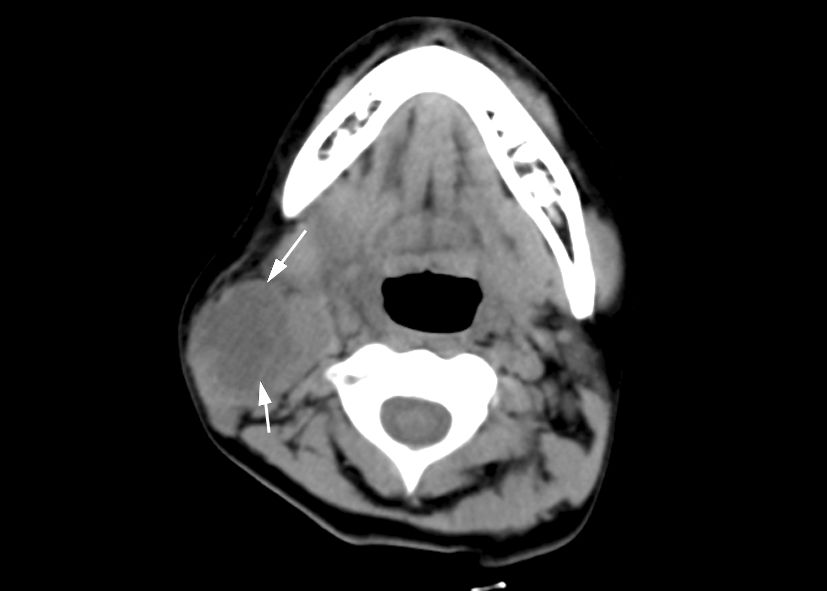
\includegraphics[width=.7\textwidth,height=\textheight,keepaspectratio]{./images/Image00173.jpg}
 \captionsetup{justification=centering}
 \caption{右侧颈部脓肿\\{\small 右侧颈部可见较大脓腔,壁厚;邻近皮下脂肪间隙及周围间隙模糊}}
 \label{fig8-6}
  \end{figure} 

\subsection{组织细胞坏死性淋巴结炎}

本病又名坏死性淋巴结炎、亚急性坏死性淋巴结炎、假淋巴瘤样增生等。本病于1972年由日本学者Kikuchi首先报道。确诊依靠病理活检和免疫组化检查。

\textbf{【病因病理】}
其病因不明,可能与病毒感染有关。如EBV、人T淋巴细胞病毒(HTLV)及巨细胞病毒(CMV)等,与诱发局部高敏反应及自身免疫有关,免疫功能异常的病人如系统性红斑狼疮(SLE)发生HNL的几率达12%~59%。据报道还与布鲁菌、耶尔森菌及弓形虫感染以及机体免疫功能紊乱,尤其是细胞毒性T细胞导致淋巴结内细胞凋亡有关。

组织学特点为淋巴结包膜完整,坏死区多局限在淋巴结的副皮质区。多表现为局限的嗜酸性纤维素样坏死物质,合并有显著的核碎屑散在分布于坏死区内,并有不典型的单核细胞。反应性免疫母细胞见于淋巴组织围绕的坏死区内,形成典型的“斑驳样”表现。罕有浆细胞及多核白细胞,有助于与猫抓热、性病淋巴肉芽肿、传染性单核细胞增多症等鉴别。

\textbf{【临床表现】}
多见于女性,男女之比约为1∶4,发病年龄11~75岁,中位年龄为30岁。多表现为无症状颈部淋巴结肿大,也可伴有发热、颈部淋巴结疼痛。实验室检查无特异性,如血白细胞可显著升高、血沉可显著增快、C反应蛋白可为阳性。30%病人可伴有多形性或药疹样皮疹,少数有恶心、呕吐、肝脾肿大和急性期外周血白细胞减少等。抗生素治疗无效,强的松等激素治疗有效;一般1~4个月后自愈。

\textbf{【CT表现】}
多为单侧颈部多发淋巴结肿大,聚集成簇、各自独立,直径多在0.5~2.5cm可达3.5cm以上(图\ref{fig8-7})。增强扫描呈均匀或不均匀强化。好发于颈静脉链及颌下淋巴结,亦可发生于纵隔、腋下、腹腔、腹膜后、肠系膜及腹股沟。国外有学者认为颈部与其他部位同时成簇出现的小淋巴结为本病的特征性表现。



\begin{figure}[!htbp]
 \centering
 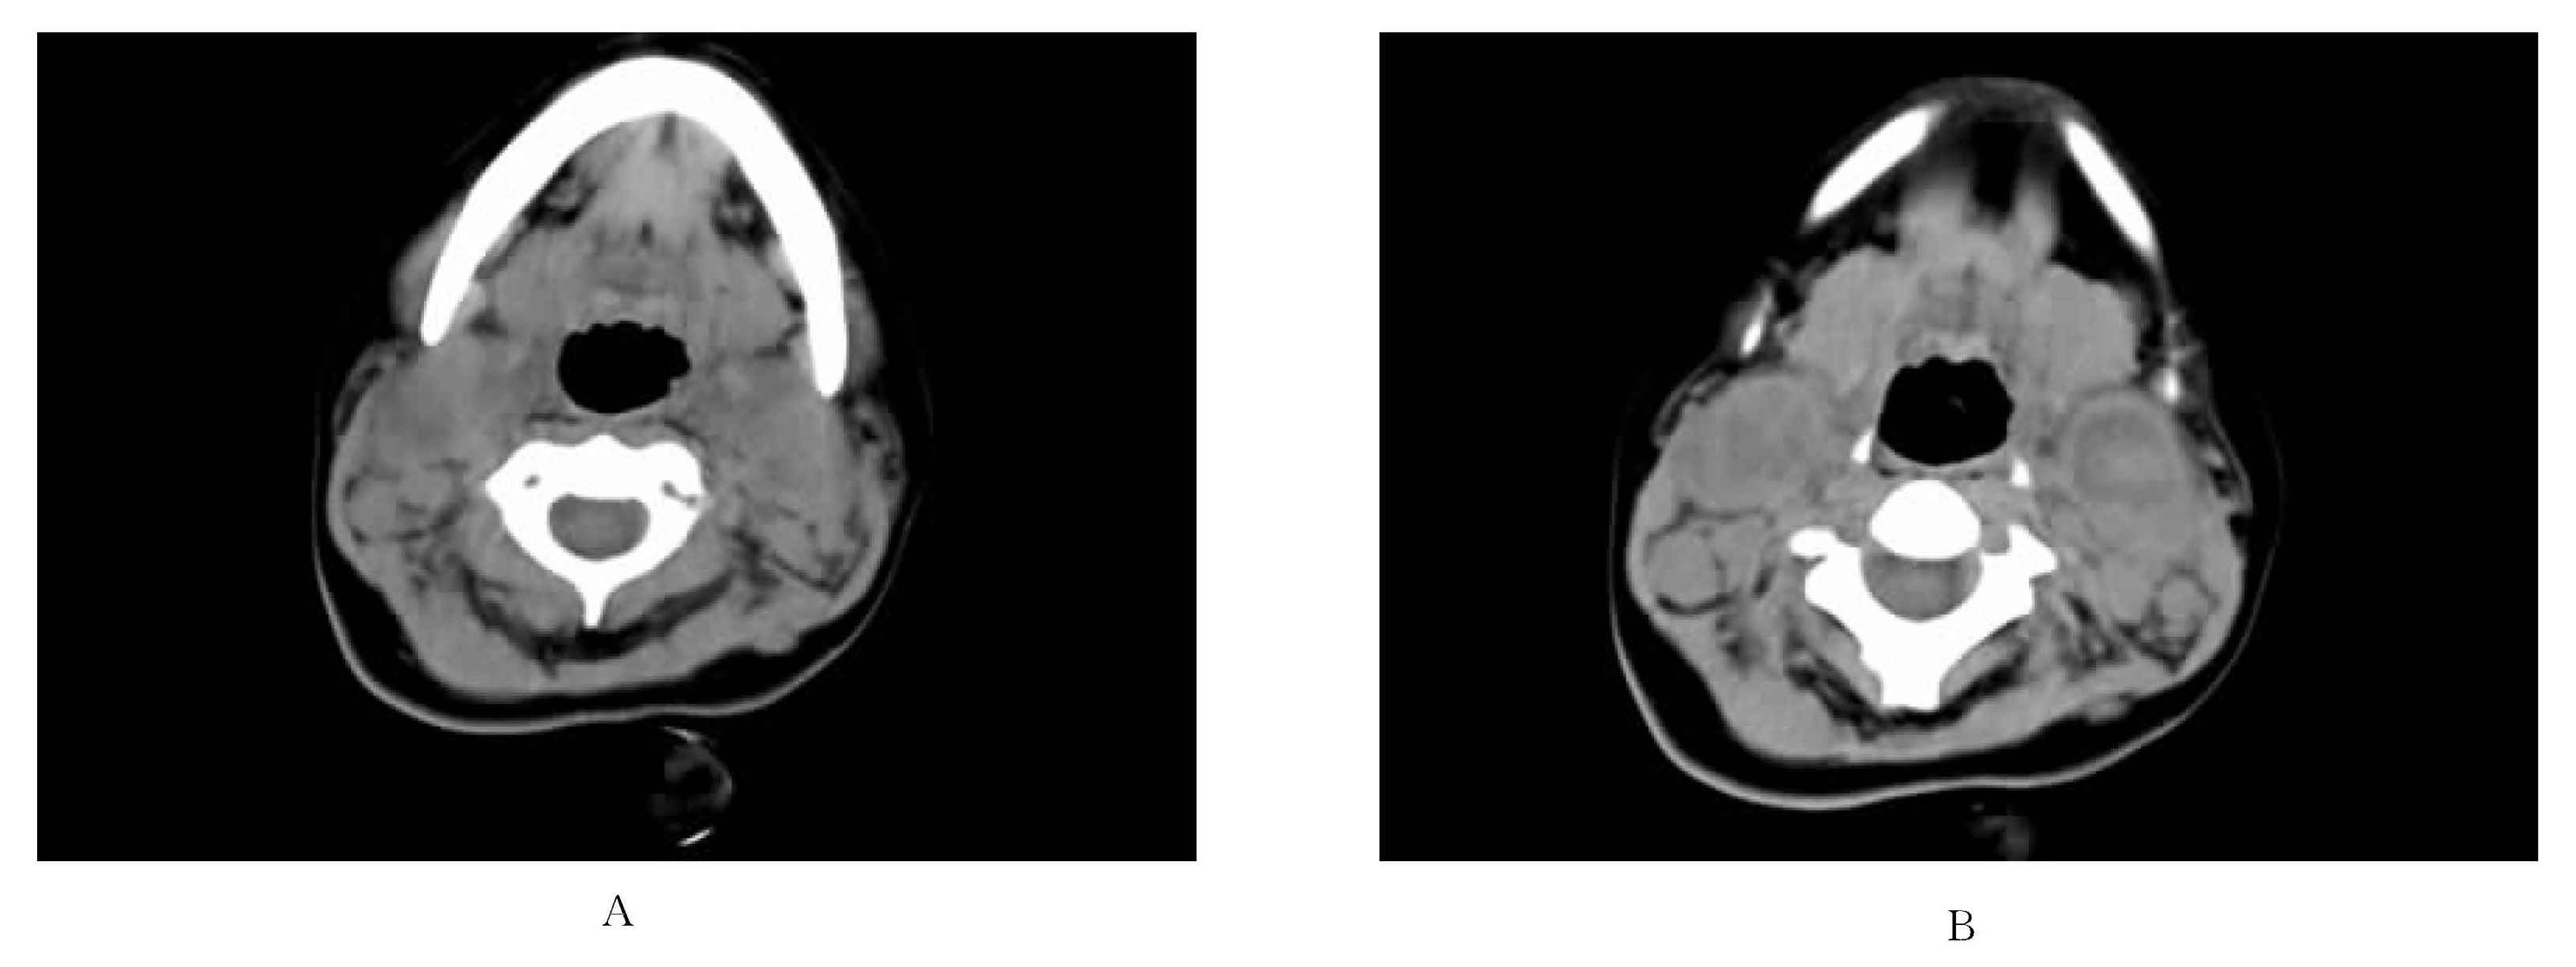
\includegraphics[width=.7\textwidth,height=\textheight,keepaspectratio]{./images/Image00174.jpg}
 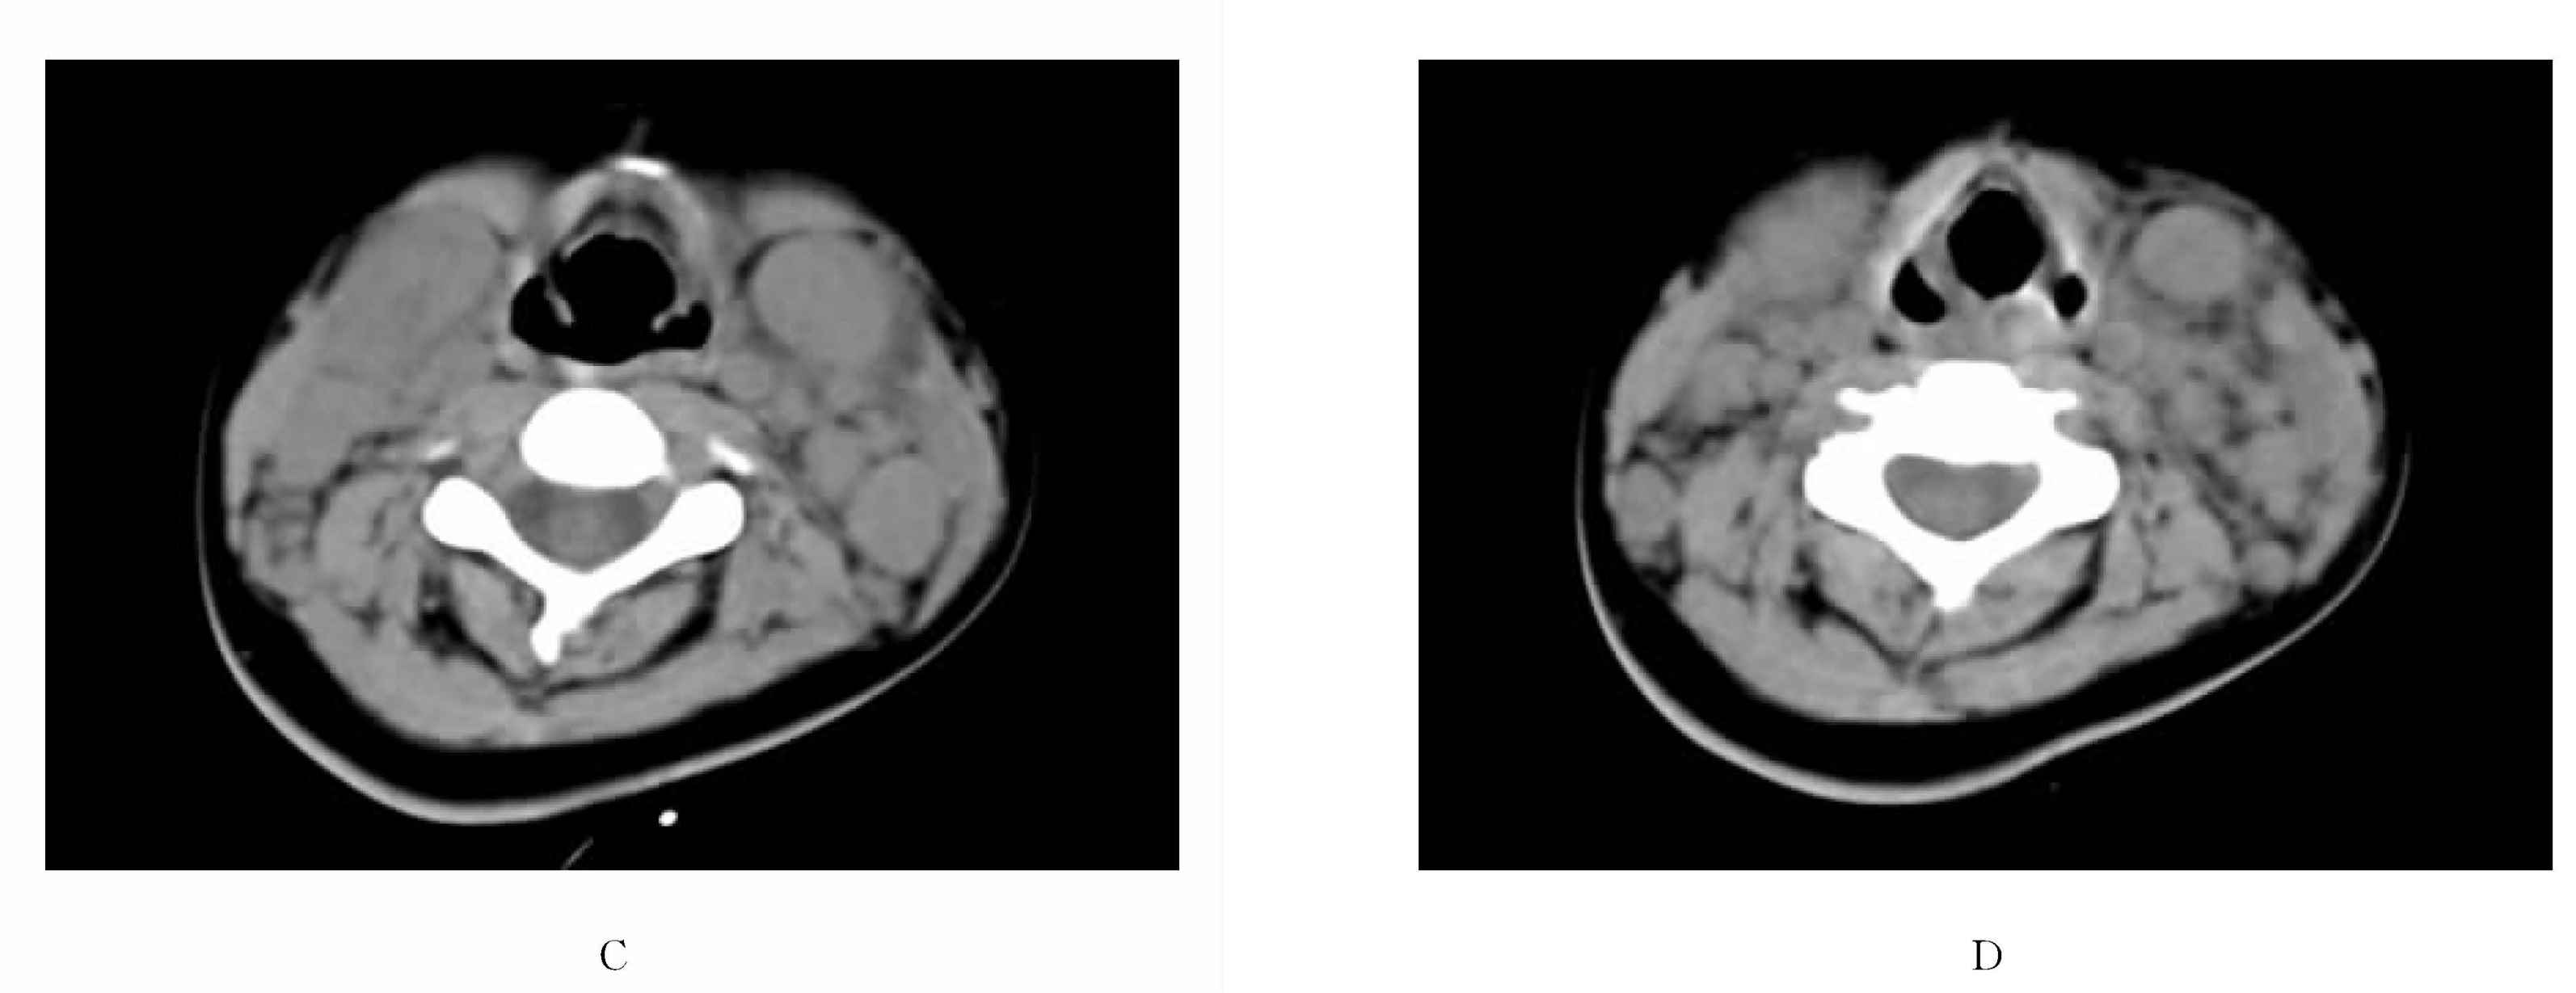
\includegraphics[width=.7\textwidth,height=\textheight,keepaspectratio]{./images/Image00175.jpg}
 \captionsetup{justification=centering}
 \caption{组织细胞坏死性淋巴结炎\\{\small 患者女性,12岁。左右颈部弥漫性分布有许多大小不一的肿大淋巴结,大者约3.5cm;部分出现液化坏死表现}}
 \label{fig8-7}
  \end{figure} 

\subsection{颈部实质性强化结节或肿块的鉴别诊断}

1.以增强后病变强化的程度分为两类:①显著强化者有:颈动脉体瘤、颈部血管瘤和颈动脉瘤;②病变轻度强化者有:神经鞘瘤、神经纤维瘤、淋巴瘤和淋巴结转移瘤。

2.颈动脉体瘤、颈部血管瘤和颈动脉瘤都以单个多见,且均显著强化。①颈动脉体瘤增强后多呈均匀性高度强化,少数可见富血管的纤维间隔呈条状或分隔状显著强化。②颈血管瘤多为海绵状血管瘤,呈多结节状强化,如平扫有钙化,尤其静脉石样钙化有助于定性。③颈动脉瘤密度及强化与颈动脉一致;有时与颈动脉体瘤鉴别困难,但颈动脉体瘤可引起颈内、外动脉之间距增大,强化幅度稍小、且稍晚于颈动脉瘤有助于鉴别。

3.神经鞘瘤、神经纤维瘤、颈淋巴瘤和颈淋巴结转移瘤均有轻度强化,以下几点有助于鉴别:①颈淋巴瘤和颈淋巴结转移瘤常为多发,而颈部神经鞘瘤和神经纤维瘤多为单个。故颈部多个结节,尤其是双侧多个,且有轻度强化者,应考虑为颈淋巴瘤或淋巴结转移瘤。颈淋巴瘤很少有坏死,而转移瘤可有坏死。故多发结节或肿块无坏死者淋巴瘤可能性大。②颈外侧部肿物单个且较大(直径>5cm),即“大而单个”,增强扫描轻度强化,且同侧颈动、静脉被推移向前或前外侧者,应多考虑为神经源性肿瘤。而颈淋巴瘤或淋巴结转移瘤虽亦可单个,但当其增大至>5cm时仍单个者少见,且同侧颈动、静脉多被推向内或内前方。③当颈外侧部见单个实质性轻度强化的小结节(直径≤3cm)时,鉴别诊断十分困难。此时,神经鞘瘤、神经纤维瘤、颈淋巴瘤和淋巴结转移瘤均有可能。④淋巴瘤可有全身其他表现,淋巴结转移瘤可有原发肿瘤病史等亦有助于鉴别。

\section{甲状腺疾病}

\subsection{异位甲状腺}

本症并不多见,是指在正常位置以外出现的甲状腺组织的统称,是先天因素所致。可分布于从口腔至膈肌的任何部位,甚至出现于腹、盆腔内。临床上较常见的是胸内甲状腺、舌甲状腺和颈部异位甲状腺。

\textbf{【病因病理】}
①舌甲状腺:系胚胎发育过程中甲状腺始基有部分或全部残留于舌根处。故可与正常部位的甲状腺共存或单独存在。单独存在者将成为体内甲状腺素的惟一来源。②胸内甲状腺:是指全部或部分位于胸骨切迹以下的甲状腺,可位于纵隔的任何部位,但以前上纵隔者最多见。胸内甲状腺又可分为完全胸内甲状腺(又称真性胸内甲状腺)和部分型胸内甲状腺。完全型与颈部甲状腺无组织学联系;部分型与颈部甲状腺相连称之为假性胸内甲状腺,可由甲状腺肿大或甲状腺异位而致。

上述异位甲状腺也可发生甲状腺肿、囊肿或肿瘤,但较少恶性。也可有甲状腺功能异常。当异位甲状腺为体内惟一甲状腺素来源时,切忌手术切除。

\textbf{【临床表现】}
无特征性。舌甲状腺部分无症状,肿块增大至一定程度可导致咽腔狭窄和吞咽困难。胸内甲状腺多无症状,压迫气管可出现咳嗽、呼吸困难或有哮喘;压迫膈神经、喉返神经、迷走神经、交感神经将出现相应症状。

\textbf{【CT表现】}

1.舌甲状腺:平扫可见舌根附近位于中线的实质性肿块,多呈圆形,边界清楚,大小不一;其密度多较软组织高且均匀,一般无钙化、囊变或坏死。增强扫描多呈均匀性明显强化。可见邻近组织受压推移甚至咽腔狭窄,但无浸润破坏。

2.胸内甲状腺:无固定位置,表现为圆形或类圆形软组织肿块,边缘多清晰,密度均匀且较高;增强扫描明显强化。部分型胸内甲状腺与颈部甲状腺组织相连有一定特征。压迫邻近组织器官有相应的表现。胸内迷走甲状腺由于位置不定极难辨认。

\subsection{甲状腺囊肿}

本病并非是一个单一的疾病,绝大多数甲状腺囊肿为良性。

\textbf{【病因病理】}
其形成主要由单纯性甲状腺肿、甲状腺瘤退变而来,单纯性囊肿少见。少数囊壁为鳞状上皮的囊肿,可能来源于化生上皮如甲状舌管及第四腮裂的残留。根据内容物性质可分为胶性囊肿、浆液性囊肿、坏死性囊肿、出血性囊肿和混合性囊肿,以前两型多见。胶性囊肿主要来源于胶性甲状腺肿;浆液性囊肿可来源于结节性甲状腺肿和甲状腺瘤退行性变。

\textbf{【临床表现】}
甲状腺部可触及柔软结节,有囊性感。囊内压力高时,触之较硬,难与实质结节鉴别。较大囊肿可有邻近结构的受压移位。

\textbf{【CT表现】}
平扫呈甲状腺区边缘清楚的近水样低密度灶;增强扫描无强化(图\ref{fig8-8})。胶质性甲状腺囊肿CT值略高于浆液性、单纯性囊肿及坏死后形成的囊肿,囊肿内出血亦使密度增高。

\begin{figure}[!htbp]
 \centering
 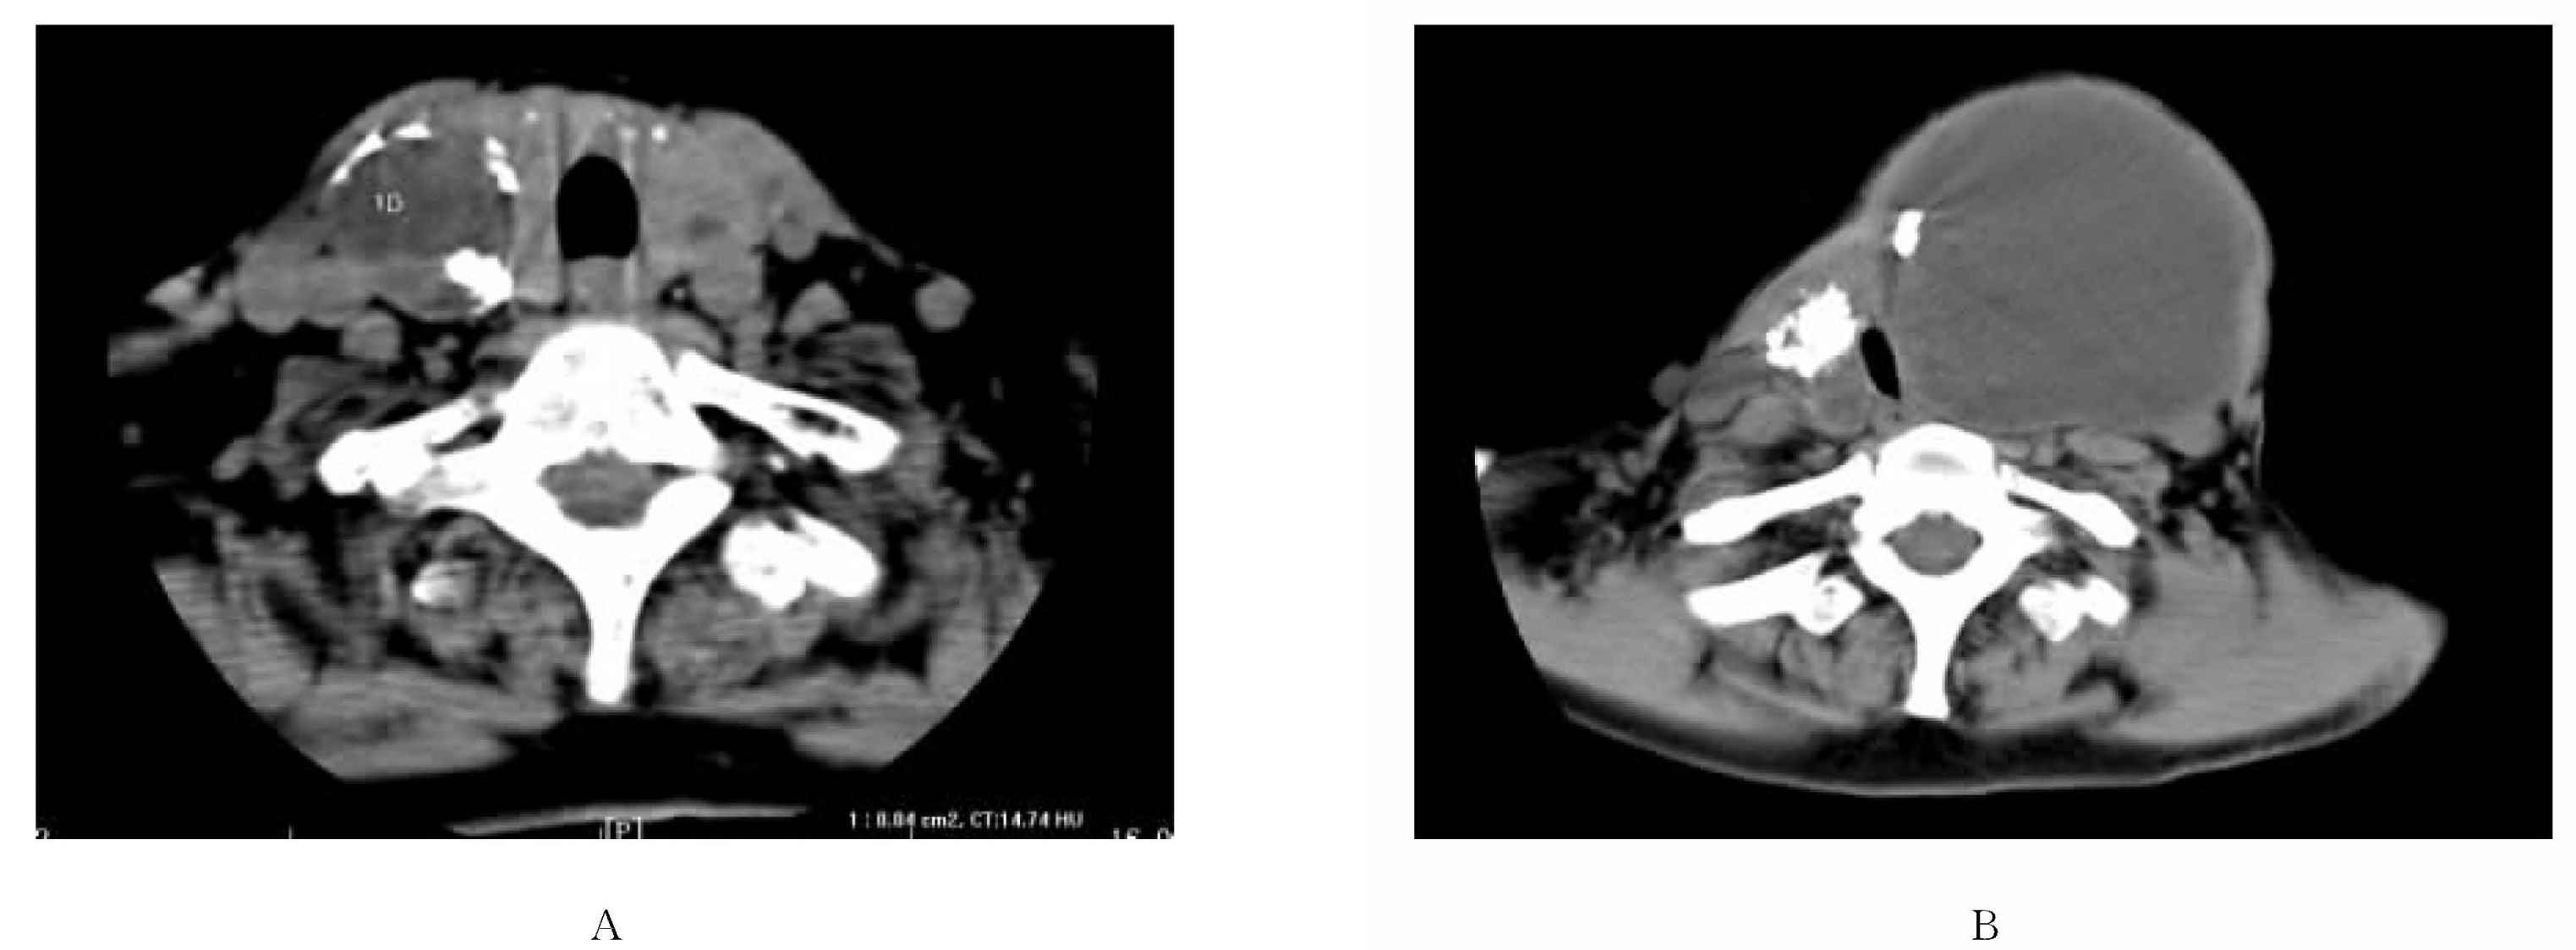
\includegraphics[width=.7\textwidth,height=\textheight,keepaspectratio]{./images/Image00176.jpg}
 \captionsetup{justification=centering}
 \caption{甲状腺囊肿\\{\small A、B非同一患者,囊肿分别位于右侧和左侧,为结节性甲状腺肿囊变所致}}
 \label{fig8-8}
  \end{figure} 

\textbf{【鉴别诊断】}
主要应与甲状腺囊腺瘤鉴别。后者周边部分构成的囊壁较厚、有强化,且内缘不及囊肿光滑锐利,是最重要的鉴别点。

\subsection{急性甲状腺炎}

甲状腺炎通常按病理及临床表现分为以下3类:①急性甲状腺炎;②亚急性甲状腺炎;③慢性甲状腺炎:又分为桥本甲状腺炎和Riedel甲状腺炎两类。甲状腺炎是由病毒、化脓性细菌、各种理化因素和自身免疫反应等引起的甲状腺炎症性改变。常伴有不同程度的全身反应。

\textbf{【病因】}
急性甲状腺炎少见。可分为化脓性和非化脓性,多由颈部化脓性细菌感染直接波及甲状腺所致。

\textbf{【临床表现】}
急性甲状腺炎表现为甲状腺局部红、肿、热、痛,重者形成脓肿,并伴有全身症状。一般无功能异常。临床易于确诊,一般无需CT检查。

\textbf{【CT表现】}
急性甲状腺炎多表现为局限性增大,边缘模糊,其内可发现低密度脓肿样改变,多有甲状腺邻近软组织的炎性改变。结合临床不难诊断。

\subsection{亚急性甲状腺炎}

本病又称为肉芽肿性甲状腺炎、巨细胞性甲状腺炎等,较常见。本病约占甲状腺疾病的5%。

\textbf{【病因病理】}
一般认为由病毒感染所致,包括流感病毒、柯萨奇病毒、腺病毒和腮腺炎病毒等,并且与HLA-B35相关。病理表现甲状腺轻度增大、水肿,甲状腺滤泡结构破坏。组织内存在许多大吞噬细胞,包括巨细胞。

\textbf{【临床表现】}
本病以40~50岁的女性多见。轻至中度甲状腺增大,局限于一叶、局部或弥漫性,且变化快,并伴疼痛。可伴有全身不适、食欲减退、肌肉疼痛、发热、心动过速、多汗等症状。少数颈部淋巴结增大。虽病程较短,且能够自行缓解,但易复发。甲状腺摄碘率下降,但T\textsubscript{3}
、T\textsubscript{4} 可一过性升高伴甲亢。

\textbf{【CT表现】}
多表现为甲状腺不对称性肿大,病灶可局限或弥漫。病变区局部密度明显降低,其边缘模糊。增强扫描可有轻度强化。

应注意结合临床与产后甲状腺炎相鉴别,后者是产后的一种亚急性自身免疫性甲状腺炎。

\subsection{慢性淋巴细胞性甲状腺炎}

本病于1912年由日本学者Hashimoto(桥本)首先报道,故称为桥本病或桥本甲状腺炎。本病为自身免疫性甲状腺炎。被分为甲状腺肿大性和甲状腺萎缩性两个临床亚型。前者甲状腺肿大;后者甲状腺萎缩并可能是前者的终末期。

\textbf{【病因病理】}
本病可能为病毒或其他理化因素所致。镜下主要表现为间质淋巴细胞浸润和滤泡上皮嗜酸性病变,可有纤维化和实质萎缩。①典型者呈弥漫性增大,有些一叶增大更著,但也可大小正常。有些呈明显的多结节外观。包膜完整、增厚,质地坚硬,易与癌混淆。但病变弥漫,与周围组织无粘连有别于癌。病变不向甲状腺外延伸,无坏死和钙化。②结节状生长者确有发生,结节的上皮性成分呈增生性改变;单个或多发结节亦可完全由嗜酸性细胞组成,但也有可能合并腺瘤。

\textbf{【临床表现】}
好发于中年女性,男女之比为1∶6~1∶20。起病隐匿,进展缓慢。常无特殊感觉,主要表现为甲状腺肿大,以峡部更著。通常约25%病例早期可有甲亢表现,大多逐渐出现甲状腺功能低下改变,少数甲状腺功能稳定。其临床特点为:病程为数月、数年或数十年;甲状腺中度增大,病程长者可有结节;大多表现为甲低、间或有甲亢。

\textbf{【CT表现】}
甲状腺两叶对称性弥漫性增大,或一叶增大更著。中等大小。密度均匀性明显减低,近软组织密度。无腺内更低密度结节影及钙化灶,边缘清楚。增强扫描呈均匀强化。以上表现可提示诊断;如临床有甲低症状或出现甲状腺自身抗体,可诊断本病。有些甲状腺密度不均匀减低,内见多个小结节,边缘呈结节外观,两叶改变大致相仿;增强扫描明显强化,结节区密度稍低,边界清晰,以上表现可考虑本病,结合临床多可确诊。但少数病例甲状腺增大不明显且密度均匀,常会造成误诊。

并发症:恶性淋巴瘤、白血病、乳头状癌和嗜酸性细胞肿瘤等,本病伴发单发结节应高度怀疑有恶变可能。

\textbf{【鉴别诊断】}
急性和亚急性甲状腺炎多有明显的临床症状和体征如发热、疼痛等易于提示诊断。但对慢性甲状腺炎的诊断尤其应慎重。桥本病应与下列疾病相鉴别。

1.弥漫性甲状腺肿:单纯弥漫性改变的桥本病与弥漫性甲状腺肿均多表现为弥漫对称性肿大,或一侧肿大更明显;密度多均一减低,腺内无结节,边缘清楚等特点,鉴别较为困难。但①应结合临床症状及体征,尤其结合化验予以鉴别。桥本病虽少数早期有甲亢症状,但最终表现为甲状腺功能低下,可与Grave病相鉴别。而单纯性弥漫性甲状腺肿,甲状腺功能多正常(但亦可有甲低表现)。②显著增大的弥漫性甲状腺肿内如因大量胶质积累(即弥漫性胶样甲状腺肿)而见多发低密度,且腺体边缘光滑,则有助于同桥本病鉴别。但如不结合临床与桥本病弥漫性改变伴多发结节亦可出现鉴别困难。③桥本病密度减低较弥漫性甲状腺肿更明显,密度与软组织相仿。④弥漫性甲状腺肿内残存之“岛状”的正常或相对正常的腺体结构常见。⑤桥本病中等大小,不及弥漫性甲状腺肿,包膜也不及后者清晰。

2.结节性甲状腺肿:多为甲状腺不对称性肿大,内见多个大小不一的低密度区,密度高低不一,可有囊变及钙化灶。可与桥本病弥漫性改变伴多发结节相鉴别。

3.甲状腺癌:多为甲状腺不对称性肿大,可见均质或不均质低密度区,可伴钙化(45%),病变可侵犯邻近结构,常有颈部淋巴结转移。但有时鉴别也较为困难。

\subsection{慢性纤维性甲状腺炎}

本病更为罕见,于1896年Riedel首先报道,故又称为Riedel甲状腺炎。

\textbf{【病理】}
甲状腺结构破坏,被纤维组织取代,可侵及周围组织。可能与硬化性胆管炎、Crohn病以及结缔组织病等免疫性疾病有相关性。

\textbf{【临床表现】}
甲状腺增大,本病累及一叶或一部分时不引起功能改变,但累及两叶时可导致甲状腺功能低下。

\textbf{【CT表现】}
无特异性。多显示甲状腺一叶或两叶增大,平扫为软组织密度。增强扫描强化不明显,对周围组织压迫明显。

\subsection{甲状腺肿的病因及分类}

\textbf{【病因】} 本病是由于下列因素导致的甲状腺非肿瘤性增生性疾病。

1.缺碘:包括①碘摄入不足:地方性甲状腺肿流行区的土壤、饮水、蔬菜、粮食中含碘量一般较非流行区低,以致碘摄入不足,是本病的主要原因;②碘需要量增加:见于儿童生长期、青春期、妊娠妇女、授乳期,或感染、创伤及寒冷等因素,使人体对甲状腺素和碘的需要量增加,在碘供应相对或绝对不足的情况下,可诱发和加重本病。

2.致甲状腺肿的物质:①某些食物如木薯含有氰基甙,在肠道内分解形成硫氰酸盐,抑制甲状腺摄碘;②饮水、土壤中某些金属离子过多,如钙和镁可以抑制碘的吸收;氟和碘在体内有拮抗作用;③某些药物如对氨水杨酸、保泰松、锂、硫氰酸盐、磺胺类及硫脲类,可影响甲状腺的吸碘及甲状腺素的合成;④长期服用含碘药物或高碘地区,由于摄碘过多,可阻碍甲状腺内碘的有机化,也可引起甲状腺肿。

3.先天性甲状腺素合成障碍:为儿童期散发性甲状腺肿的一种少见原因。主要由于先天性的某些甲状腺合成酶缺陷所致。

\textbf{【分类】}

1.根据有无功能亢进可分为:①非毒性甲状腺肿:亦称为单纯性甲状腺肿。无甲亢表现,甚至部分甲低,出现呆小病改变。②毒性甲状腺肿:有甲亢表现。

2.根据增生的形态学改变可分为:①弥漫性甲状腺肿;②结节性甲状腺肿。

3.单纯性甲状腺肿根据流行情况分为:①地方性:主要因碘摄入不足所致;②散发性:主要因碘的需要量增加所致。

\subsection{单纯性甲状腺肿}

\textbf{【发病机理】}
体内甲状腺素绝对或相对不足导致甲状腺滤泡上皮代偿性增生肥大,从而致甲状腺呈弥漫性增大,以使其分泌的甲状腺素能代偿性满足机体的需要,维持正常代谢。随着病程的延长将出现不同的病理改变。

\textbf{【病理】} 其病理过程分为以下3期:

1.增生期(弥漫性甲状腺肿):早期为滤泡均匀增生,导致腺体弥漫性增大,表面光滑。镜下见甲状腺充血,滤泡上皮呈立方状或柱状,并伴有小型滤泡增生。此期代偿功能增强。代偿后的增生上皮又可恢复原状(复旧)。

2.胶质储积期(弥漫性胶样甲状腺肿):长期持续缺碘,滤泡上皮反复增生、又复旧,小型滤泡变大。腔内充满胶样物质,使上皮细胞受压变扁平。甲状腺呈均匀弥漫性增大,包膜完整,表面光滑,质地较硬。

3.结节期(结节性甲状腺肿):在流行区较常见。由于甲状腺内不同部位的滤泡上皮增生与复旧变化不同步,逐渐发展成大小不等的结节,结节可出血、坏死、囊变及钙化等。镜下形态多样,有的滤泡高度扩张,腔内充满胶质,甚至形成囊肿;有的滤泡甚小,几乎不含胶质;还有的滤泡上皮细胞向腔内呈乳头状增生,这种改变易发生恶变。

\textbf{【临床表现】}
可发病于任何年龄,但以10~25岁多见,男女之比为1∶1.5~1∶3。以甲状腺增大而无全身症状为特征性表现。早期弥漫性增大,久而形成结节。肿块随吞咽活动、质软、表面光滑。有广泛钙化时,质地变硬。但活动度仍良好。肿块大者可有压迫症状,如压迫气管可有呼吸困难等症状。

\textbf{【CT表现】}

1.增生期(弥漫性甲状腺肿):即早期表现。甲状腺比较均匀的弥漫性肿大,大致形态正常。增强扫描明显强化。

2.胶质储存期(弥漫性胶样甲状腺肿):甲状腺密度可不均匀或减低,其内可见多发更低密度灶。增强扫描低密度灶更清晰且可无强化。

3.结节期(结节性甲状腺肿):甲状腺多呈明显不均匀增大,形态轮廓发生改变,并对邻近器官造成推移;其结节多呈大小不等的多个边界清楚的低密度灶,结节坏死、囊变时,密度明显减低,且不强化,钙化常见(图\ref{fig8-9})。结节出血时原肿块迅速增大,其内密度增高。当发生恶变时肿块向邻近器官浸润,周围淋巴结增大。甲状腺肿大亦可向下伸延至胸骨后,形成胸骨后甲状腺肿,它同样亦可出现低密度结节及其囊变、出血和钙化。

\begin{figure}[!htbp]
 \centering
 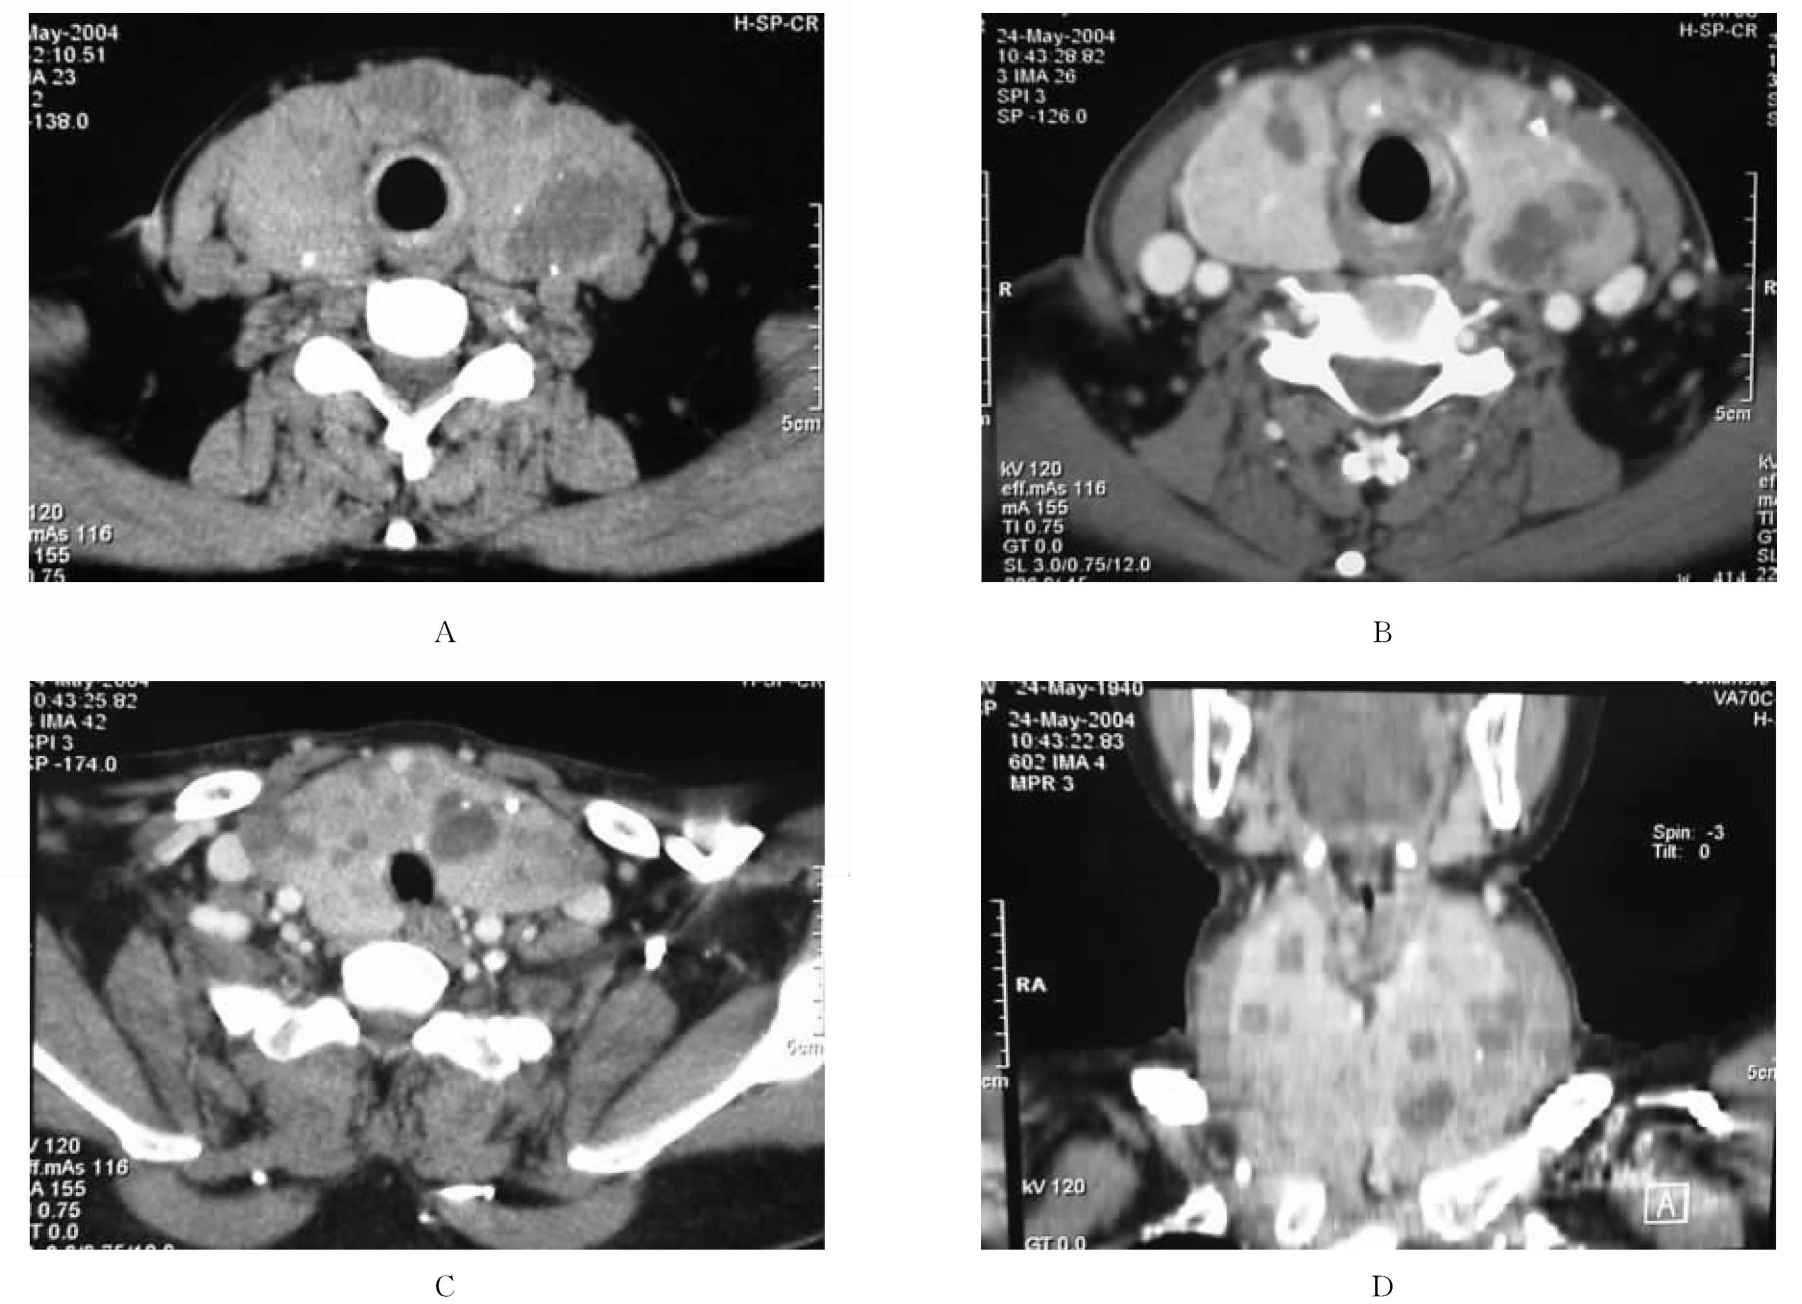
\includegraphics[width=.7\textwidth,height=\textheight,keepaspectratio]{./images/Image00177.jpg}
 \captionsetup{justification=centering}
 \caption{结节性甲状腺肿\\{\small A~D为同一患者,甲状腺弥漫性增大,密度不均且有粗颗粒状钙化;增强扫描其内有许多大小不等的低密度结节,结节边缘清晰光整}}
 \label{fig8-9}
  \end{figure} 

前两期形态学称为弥漫性甲状腺肿,结节期即结节性甲状腺肿。总之,对甲状腺肿的影像学检查以超声最为便捷,且可清晰显示,结合病史及检验等不难诊断。但影像学并无特异性,尤其是前两期(弥漫性甲状腺肿大)与Graves病、甲状腺炎等所致的甲状腺弥漫性增大相类似,鉴别主要依靠临床、实验室检查。

\subsection{弥漫性甲状腺肿伴甲亢(Graves病)}

甲亢是由多种原因引起的甲状腺素分泌过多所致的一种内分泌疾病,其病因很多,如甲状腺性甲亢(包括Graves病、多结节性甲状腺肿伴甲亢、自主性高功能性甲状腺腺瘤、新生儿甲亢、长期大量摄碘所致的碘源性甲亢、由于分泌甲状腺素过多所致的滤泡性甲状腺癌)、垂体性甲亢、异源性TSH综合征、卵巢甲状腺肿等。Graves病为甲亢中最常见的一类,临床所说的甲亢通常指这一种,因常伴有突眼故又称为突眼性甲状腺肿。本病可能主要与自身免疫反应有密切关系。

\textbf{【病理】}
甲状腺弥漫性增大,切面呈灰白色,质实如肌肉,胶质少。镜下除可见滤泡上皮细胞呈高柱状增生、常有乳头形成外,与非毒性弥漫性甲状腺肿的主要区别为滤泡内胶质减少、周边可见吸收空泡,无胶性囊肿形成;间质血管增生、明显充血,大量淋巴细胞浸润,并形成淋巴滤泡。此外,还可出现全身淋巴组织增生、胸腺肥大、骨质增生、骨骼肌(特别是股四头肌)变性,以及肝脂肪变或肝坏死、心脏肥大扩张等改变。

\textbf{【临床表现】}
多见于20~40岁女性,男女之比约1∶4~1∶6。主要表现为甲状腺肿大、高代谢症群和眼球突出三大症状,血中T\textsubscript{3}
、T\textsubscript{4} 升高。

\textbf{【CT表现】}
甲状腺弥漫性增大,边缘清楚,密度较均匀性减低。可有轻度强化。明显增大者可有气管受压表现。

\subsection{甲状腺腺瘤}

甲状腺良性肿瘤约占90%,以甲状腺腺瘤多见。甲状腺腺瘤又分为乳头状腺瘤、滤泡性腺瘤(又分为单纯性腺瘤、胶样腺瘤、嗜酸性细胞腺瘤)和不典型腺瘤;少见的甲状腺良性肿瘤有畸胎瘤、血管瘤及平滑肌瘤等。

\textbf{【病理】}
甲状腺腺瘤一般为单发的圆形或椭圆形肿块,包膜完整。肿瘤较大时,可出血、坏死、囊变、钙化和恶变。滤泡性腺瘤多见,为实性。乳头状腺瘤少见,多呈囊性,内为胶质成分,故又可称为乳头状囊腺瘤(应注意与高分化乳头状腺癌相鉴别)。不典型腺瘤更少见。

\textbf{【临床表现】}
好发于20~40岁,女性多于男性,男女之比约1∶2~1∶4。多无自觉症状。肿块较大时可产生邻近器官受压症状,但无侵犯表现。部分病例可恶变,亦可转化为毒性甲状腺腺瘤。

\textbf{【CT表现】}
平扫可见甲状腺内低密度灶,边缘光滑锐利、密度均匀;大小多在1~5cm之间;多为单个(图\ref{fig8-10})。少数瘤体内有颗粒状、斑片状钙化;出血可呈高密度血液表现。增强扫描示病灶有强化,但多不及甲状腺实质增强明显;实质性肿瘤较小时强化均匀,较大时强化不均;囊性腺瘤则表现为周边部分实质呈厚壁明显强化。增强后腺瘤与邻近组织界限更清晰。

\begin{figure}[!htbp]
 \centering
 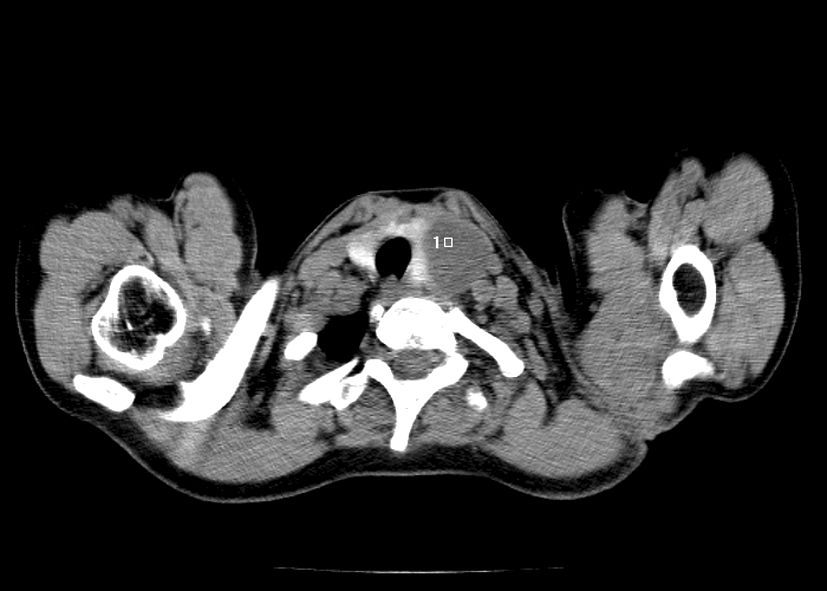
\includegraphics[width=.7\textwidth,height=\textheight,keepaspectratio]{./images/Image00178.jpg}
 \captionsetup{justification=centering}
 \caption{甲状腺腺瘤\\{\small 左侧甲状腺有圆形低密度灶,边缘光滑}}
 \label{fig8-10}
  \end{figure} 

\textbf{【鉴别诊断】}
结节性甲状腺肿的甲状腺多呈明显不均匀增大,轮廓不规整,其内有多个大小不等的、边界较清楚的低密度灶,常见钙化。而甲状腺腺瘤一般为单发,周围甲状腺组织密度正常,肿瘤较小时甲状腺形态亦正常,肿瘤大时仅见局限性甲状腺增大外突,故有别于结节性甲状腺肿。B超对鉴别诊断应优于CT。

\subsection{甲状腺癌}

甲状腺恶性肿瘤约占10%,包括起源于实质的甲状腺癌和间质的肉瘤,以甲状腺癌多见。甲状腺癌又分为乳头状腺癌、滤泡状甲状腺癌、未分化癌、髓样癌;少见的恶性肿瘤有淋巴瘤、转移瘤、类癌和肉瘤等。

\textbf{【病理】}
甲状腺癌最常见的为乳头状腺癌,约占甲状腺癌的62%。多无包膜或包膜不完整,与正常甲状腺组织分界不清,常有纤维化、钙化(由于40%~50%的乳头状癌由沙砾体,细颗粒状钙化可能与其相关)。部分囊性变即囊性乳头状癌(约占乳头状癌的5%),囊内有棕色液体。滤泡状腺癌约占23%,肿瘤有完整包膜,较大者常突破包膜向周围侵犯。其他还有未分化癌(约占6%)及髓样癌等。

\textbf{【临床表现】}
多见于青壮年女性,男女之比约为1∶2~1∶3。多为单发,少数为双侧发病或多发。肿块质地坚硬,边缘不清,活动度差。可产生邻近器官受压、受侵症状。多无明显其他症状,少数有甲亢。颈淋巴结转移多发生于未分化癌。

\textbf{【CT表现】}
平扫可见甲状腺区不规则或分叶状不均匀低密度软组织肿块,与周围界限不清;病侧甲状腺增大或双侧不对称增大;瘤体内可见砂粒状或斑块样钙化(30%~50%),有文献认为细颗粒状钙化有特征性;肿瘤内出血时密度增高(图\ref{fig8-11})。增强扫描病变有不同程度强化,但低于正常甲状腺组织。晚期可见邻近器官(如气管、食管、颈动脉)受侵和局部淋巴结转移的表现。

\begin{figure}[!htbp]
 \centering
 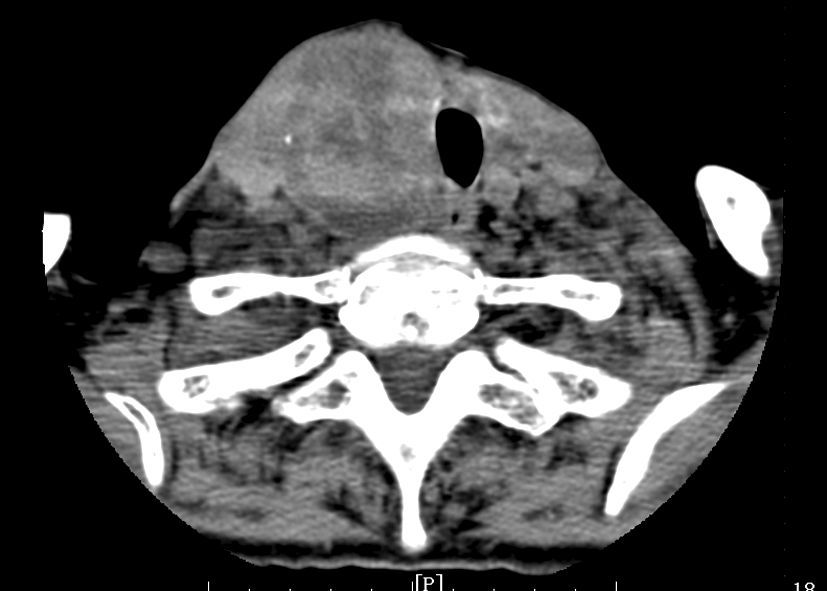
\includegraphics[width=.7\textwidth,height=\textheight,keepaspectratio]{./images/Image00179.jpg}
 \captionsetup{justification=centering}
 \caption{甲状腺癌\\{\small 病变以右侧甲状腺为主。甲状腺密度不均,其内有许多不规则低密度灶,甲状腺边缘有“半岛状”瘤结节突出,局部包膜有中断即“残圈”征}}
 \label{fig8-11}
  \end{figure} 

由于肿瘤向包膜外浸润的深度不同可形成不规则的“半岛状”瘤结节。肿瘤侵及或突破腺体边缘的包膜或假包膜,形成瘤周“残圈”征象具有特征性。囊内钙化性壁结节、囊壁厚薄不均,壁结节周围可见多个小囊与之相连,小囊间有分隔,分隔粗细不均是囊性乳头状癌的主要征象。

直径1cm以下者(隐匿性甲状腺癌)多难以显示,也可仅见钙化灶、转移淋巴结,而难以诊断。

总之,甲状腺癌多表现为低密度,密度不均,边缘模糊且不规则。细颗粒状钙化(乳头状癌多见)、瘤周“半岛状”瘤结节及“残圈”征是其特征性表现。囊内乳头状壁结节和囊内钙化性壁结节是囊性乳头状癌的特征。

\textbf{【鉴别诊断】}
①甲状腺瘤与较小的结节状癌肿可表现相似。但前者边界清、有包膜,钙化相对少见;可见瘤周完整强化环,腺体包膜完整,无颈部淋巴结转移。②慢性甲状腺炎及弥漫性甲状腺肿与周围界限较清晰,且多呈对称性增大。③结节性甲状腺肿内有多个界限清晰的低密度结节,密度不均、钙化粗大;部分边缘模糊,可见壁结节,与正常腺体同步强化;腺体包膜完整,无颈部淋巴结转移。亦与甲状腺癌有别。④淋巴瘤以弥漫肿大型多见,单发或多发结节型少见。病灶密度多均匀,坏死和钙化少见或无。与密度不均的甲状腺癌有别。但有时甲状腺癌与上述疾病鉴别较为困难,需依据B超、核素扫描等联合诊断和鉴别。

\subsection{原发性甲状腺恶性淋巴瘤}

本病少见,约占甲状腺恶性肿瘤的2.5%~5.0%。是一种与自身免疫缺陷相关的疾病。

\textbf{【病理】}
国内报道1组均为B细胞来源的非何杰金淋巴瘤(NHL)。肿瘤可侵及一叶或两叶。本病多在桥本甲状腺炎的基础上发生,可能为桥本甲状腺炎激活B细胞分泌自身抗体,导致甲状腺的淋巴组织增生,继而发生恶变的结果。

\textbf{【临床表现】}
好发于老年女性,平均年龄60~70岁。主要表现为颈部肿块。尤其以往有桥本甲状腺炎病史,近期甲状腺突然增大者,应注意本病的诊断。其诊断标准为:①组织学证实为甲状腺的淋巴瘤;②除颈部见区域淋巴结肿大受累外,全身其他部位未见肿大淋巴结。本病目前多采用放、化疗治疗。

\textbf{【CT表现】}
以弥漫肿大型多见(占67%),单发结节型或多发结节型少见。弥漫肿大型表现为一叶或两叶腺体被低密度病变代替,密度均匀。单发结节型表现为密度均匀的低密度结节。多发结节型表现为甲状腺体积增大,其内有多个低密度结节。多数文献报道肿瘤密度多均匀,坏死和钙化少见或无;增强扫描强化不显著。本病可有周围组织侵犯,但发生率低。颈部淋巴结可受累,淋巴结的形态和强化各异。

国内外文献报道约80%在桥本甲状腺炎的基础上发生。故对于年龄>60岁的女性患者,有桥本甲状腺炎病史且近期甲状腺突然增大者,CT表现甲状腺弥漫性增大,密度均匀,强化不显著,应考虑恶性淋巴瘤可能。

\textbf{【鉴别诊断】}
应注意与桥本甲状腺炎、亚急性甲状腺炎、弥漫性甲状腺肿及甲状腺癌鉴别,但鉴别有一定困难。一般认为,密度不均、并出现坏死液化、半岛状瘤结节、细颗粒状钙化、边缘不清楚在甲状腺癌多见。而淋巴瘤密度均匀,坏死液化极少见。

\section{甲状旁腺疾病}

\subsection{甲状旁腺功能亢进的病因和分类}

本病可分为以下4类:

1.原发性:病因尚不十分清楚,常由甲状旁腺腺瘤、增生或腺癌引起甲状旁腺激素分泌过多,导致高血钙、低血磷、尿钙磷增多、骨损害及肾结石等表现。以腺瘤多见,占80%~87%;其次为增生,约占15%;腺癌少见,为0.5%~2%。

2.继发性:是由于慢性肾功能不全、维生素D缺乏或抵抗,以及妊娠、哺乳等情况下,甲状旁腺受低血钙、低血镁或高血磷的刺激增生而分泌过量的甲状旁腺激素,以提高血钙、血镁和降低血磷的一种慢性代偿性变化。此外,继发性甲状旁腺功能亢进症的病因还包括各种原因所致的骨软化症、甲状腺髓样癌分泌过多的降钙素、假性甲状旁腺功能低下、皮质醇增多症以及某些药物所致的钙、磷代谢紊乱。影像学改变有:骨质疏松、骨软化、纤维性骨炎、骨质硬化等。

3.三发性:是指在继发性甲状旁腺功能亢进的基础上,甲状旁腺对各种刺激因素反应过度或腺体受到持久性刺激增生肥大,继续发展导致一个或几个腺体由增生转变为腺瘤并呈现分泌功能自主性。会引起明显的纤维性骨炎。

4.假性:于1941年由Albright首次报道,是异位分泌综合征的一种。一般指除甲状旁腺以外的某器官,尤其是肺、肝、肾、胰腺等组织的肿瘤,分泌一种或数种升血钙的活性物质所致的疾病。

\subsection{甲状旁腺腺瘤和增生}

甲状旁腺占位性病变较少见,其中较为常见的为腺瘤,部分为增生,腺癌极少见。

\textbf{【病理】}
①甲状旁腺腺瘤:绝大多数为单发,占90%以上;少数为多发或累及多个腺体。一般好发于下部甲状旁腺(占70%),直径多在5cm以下。肿瘤和增生可并存。镜下见瘤细胞多数属主细胞,也可由透明细胞组成。肿瘤多有完整包膜,可有囊变、出血、坏死、钙化。②增生:主要为主细胞增生和多个腺体受累。无包膜,可形成假包膜,并可转变为腺瘤。

\textbf{【临床表现】}
腺瘤和增生多见于30岁以上女性。早期症状不典型。出现甲状旁腺功能亢进后可出现相应症状和化验结果的改变。高钙血症伴低磷血症是原发性甲状旁腺功能亢进的最重要依据之一。肿块较大者可触及肿块并可出现局部压迫症状,如喉返神经受压出现声音嘶哑等。

\textbf{【CT表现】}

1.甲状旁腺腺瘤:位于甲状腺后方、颈动脉和食管之间,也可位于气管食管旁沟内,部分位于甲状腺下内侧或完全被甲状腺包埋。一般为单侧。呈结节状,密度均匀,边缘清楚。增强扫描明显强化,但不及血管和甲状腺,且下降迟缓。肿瘤较大时可有坏死、囊变;也可钙化,但少见。异位的甲状旁腺腺瘤可位于颈根处、前上纵隔或胸骨后。

2.甲状旁腺增生:虽有增生,但腺体较小时很难显示,一般直径>10mm才能显示。甲状旁腺增生一般4个腺体都增生,但往往大小不同,以某一个增生为主,故需仔细观察以便与腺瘤鉴别。但与多发腺瘤鉴别困难。

\subsection{甲状旁腺腺癌}

本病极少见,生长缓慢,晚期才出现转移。

\textbf{【临床表现】}
以中老年男性多见。可触及肿块,喉返神经麻痹时可有声音嘶哑的症状。亦可有甲状旁腺功能亢进(原发性)的症状和化验结果的改变。故与甲状旁腺腺瘤和增生有相同之处。

\textbf{【CT表现】}
呈界限不清的低密度肿块,并可侵及邻近组织和器官,局部淋巴结可见转移。甲状旁腺腺癌较易发生钙化,如发现甲状旁腺肿物内钙化者,应怀疑癌的可能。但在无局部淋巴结转移和远处转移的情况下,很难与甲状旁腺腺瘤鉴别。

\subsection{甲状旁腺功能减退症}

本病可分为两类:①特发性:有家族性和散发性两种,病因不明,部分学者认为是自身免疫性疾病;②继发性:为甲状腺手术损伤、摘除了甲状旁腺等原因所致。

\textbf{【病理】}
本病脑内钙化的病理机制尚不明了。可能与低血钙时血管通透性增高有关;也可能是由于脑组织发生病理性水潴留,以致钙盐在脑组织内沉积发生钙化。另外高血磷促使钙离子自骨到软组织内沉积。由于基底节区毛细血管丰富、纵横交错、排列密集,故钙质易于沉着。本病的骨骼改变与破骨细胞活动停止或减弱、肾小管对磷的重吸收增多有关,以致尿排磷量减少、血磷升高、血钙降低。因由骨骼移向血中的钙和磷都减少,以致骨骼致密。

\textbf{【临床表现】}
其症状和体征均与低血钙有关。以手足抽搐最具特征性,可以癫痫(特别是患儿)为首发症状。手足抽搐发作前有手、脚及口周麻木,还可有呼吸困难。可有智能低下(10岁以前不同程度的存在),还可有精神症状如抑郁症。胃肠道症状表现为恶心、呕吐和腹泻。实验室检查血钙降低、血磷增高。部分病例有脑电图异常。

\textbf{【CT表现】}
脑部表现为双侧基底节、丘脑、小脑、齿状核、大脑皮质下及皮髓质交界区对称性高密度钙化灶,内囊不受累;钙化常多发、大小不一,呈斑片状、月芽状、点状、条状等(图\ref{fig8-12})。本病脑内钙化率约93%。

\begin{figure}[!htbp]
 \centering
 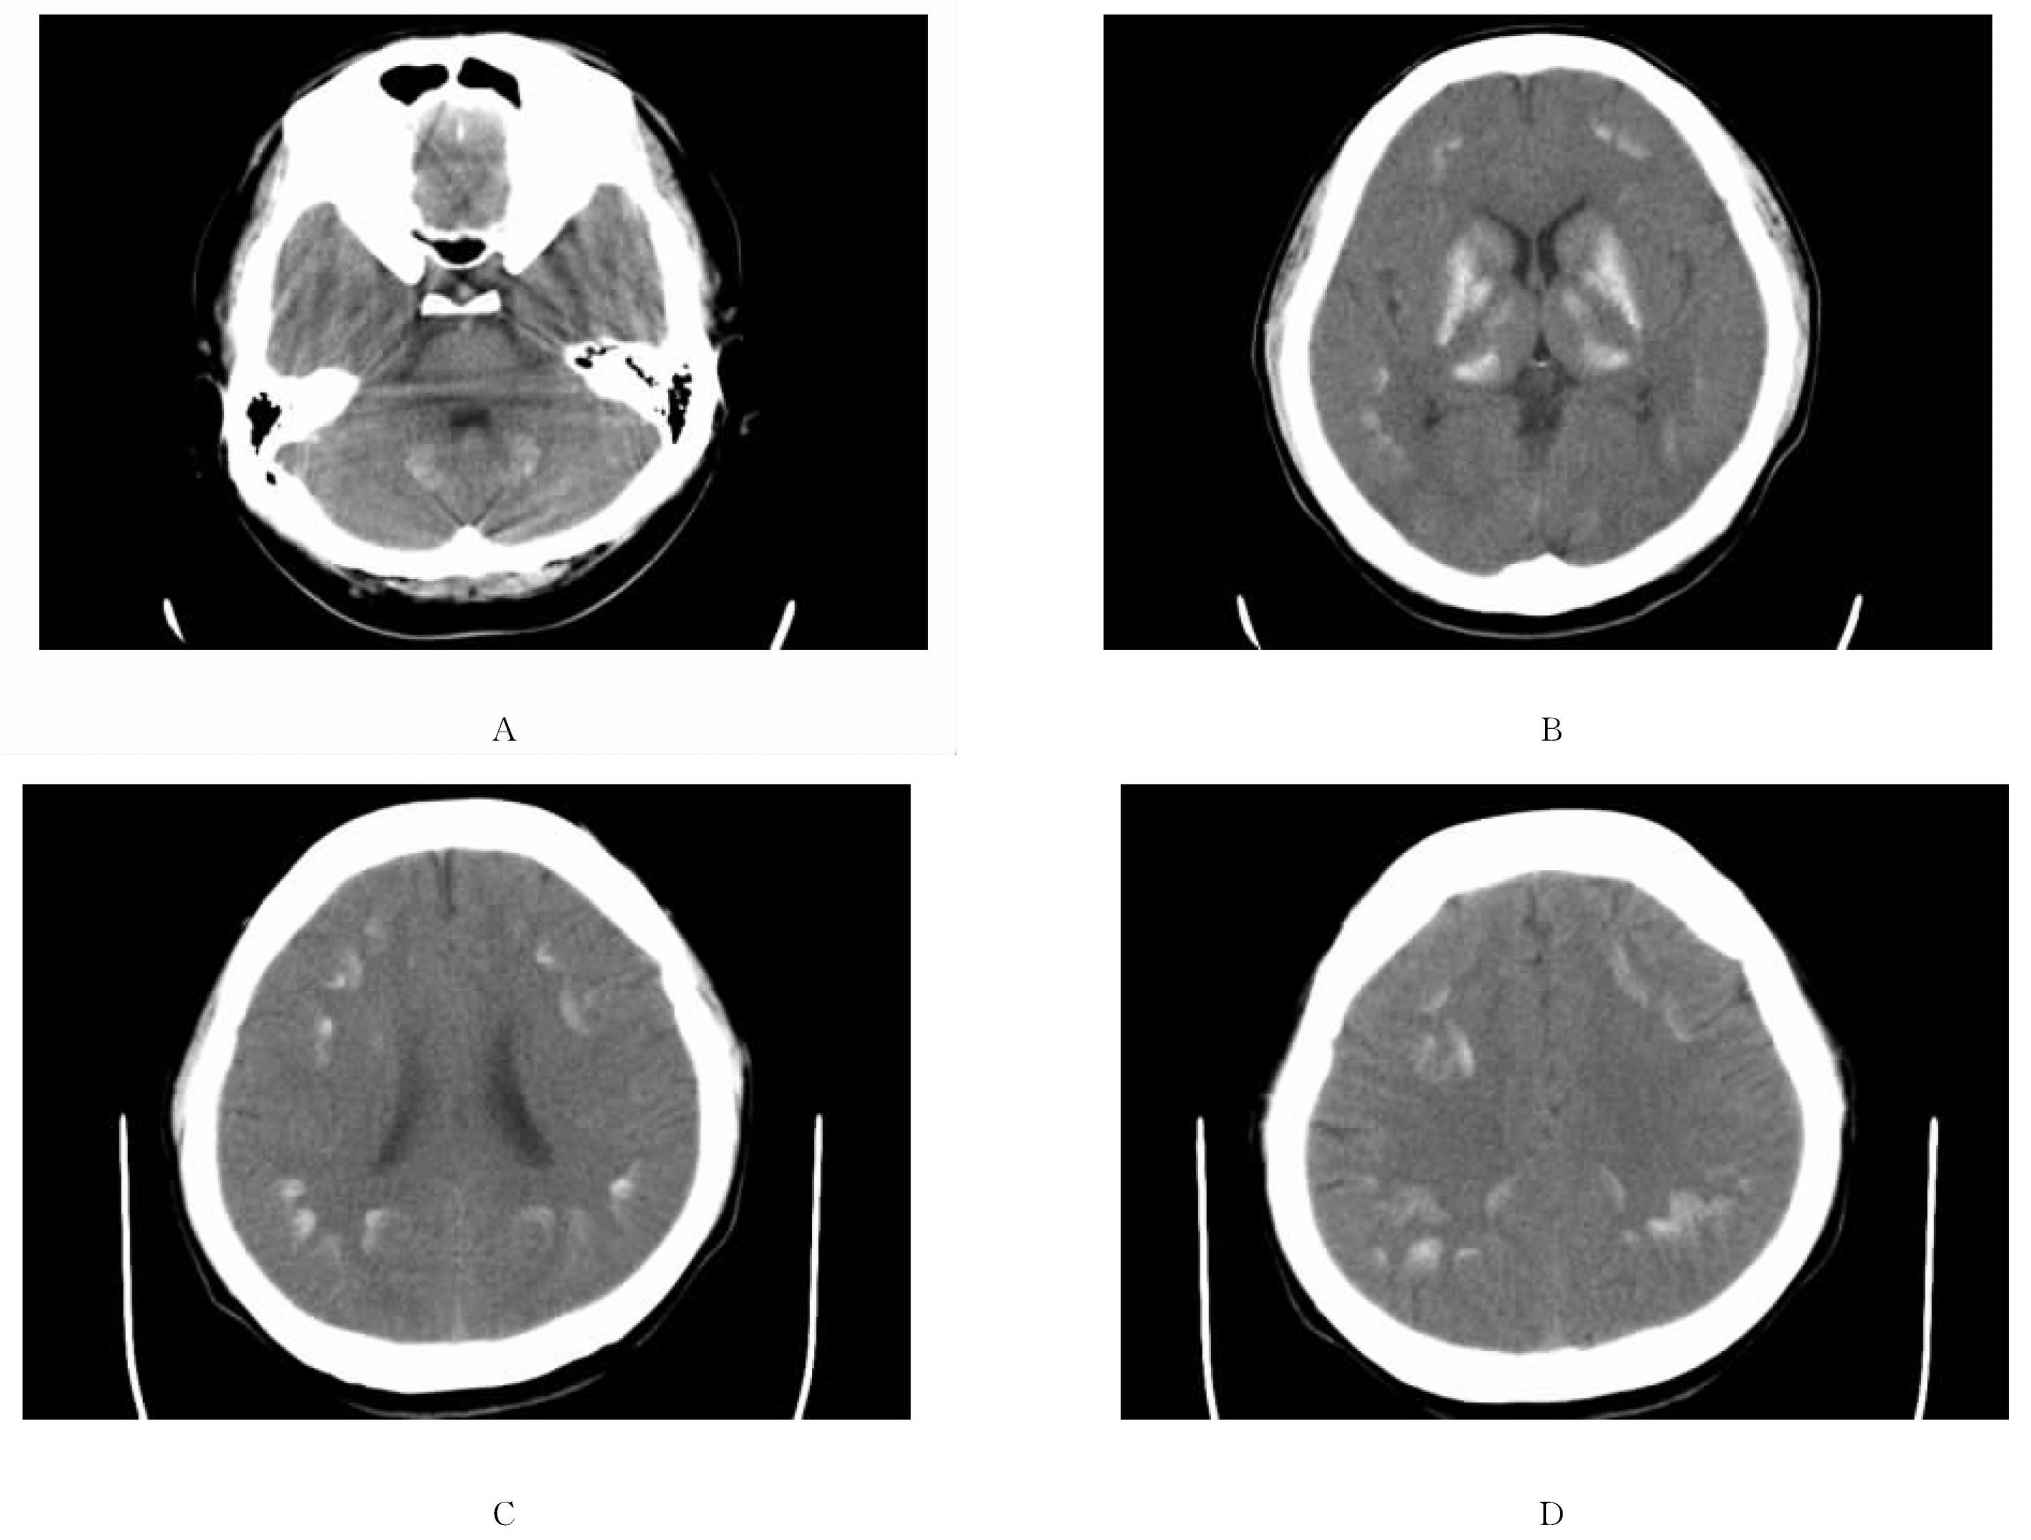
\includegraphics[width=.7\textwidth,height=\textheight,keepaspectratio]{./images/Image00180.jpg}
 \captionsetup{justification=centering}
 \caption{甲状旁腺功能减退\\{\small A~D为同一特发性患者,男14岁。小脑齿状核、左右侧基底核、左右侧丘脑、皮髓质交界处广泛对称性钙化}}
 \label{fig8-12}
  \end{figure} 

此外,平片可见骨密度普遍增高。

\textbf{【鉴别诊断】}

1.假性甲状旁腺功能减退症:本病症状、体征及实验室检查都与甲状旁腺功能减退症完全一样,但经注射甲状旁腺激素并不能奏效。可能系骨骼对甲状旁腺激素不反应而发病。患者有明显的发育异常、智力减退、短肢、面圆。慢性低血钙可并发肌肉、喉、手足或全身痉挛。骨骼有短指(趾)畸形,以第四、第五掌骨为著;有异常牙发生。关节周围软组织、颅内基底节可有钙化。

2.假-假性甲状旁腺功能减退症:本病与假性甲状旁腺功能减退症大致相同,惟其血清钙和磷都正常,无抽搐。以软组织钙化为主,极少发生基底节钙化。骨骼变化可伴有多发性家族性外生骨疣、Turner综合征,但无异常牙发生。

\protect\hypertarget{text00016.html}{}{}

